\documentclass[11pt,titlepage]{article}

\usepackage[sort&compress]{natbib}
\bibliographystyle{unsrt}
\usepackage{color}
\usepackage{graphicx}
\graphicspath{{figs/}}
%\usepackage{booktabs}
\usepackage{tabularx}
%\usepackage{mathptmx}
\usepackage{amssymb}
\usepackage{amsmath}
\usepackage{authblk}
\usepackage[margin=1in]{geometry}
\usepackage[hidelinks=true]{hyperref}

\newcommand{\todo}[1]{\textbf{$\star \star$ {#1} $\star \star$}}
\newcommand{\PNNLaffil}{$\star$}
\newcommand{\UCBaffil}{$\dagger$}
\newcommand{\UMaffil}{$\ddagger$}
\newcommand{\SMUaffil}{$\S$}
\newcommand{\FLaffil}{$\|$}
\newcommand{\Novoaffil}{$\P$}
\newcommand{\UCSDaffil}{$\Delta$}
\newcommand{\CUNYaffil}{$\diamond$}
\newcommand{\PIaffil}{$\circ$}

\begin{document}

\title{Improvements to the APBS biomolecular solvation software suite}
% \keywords{electrostatics, solvation, implicit solvent, p$K_a$, titration, software}

\author[\PNNLaffil]{Elizabeth~Jurrus}
\author[\PNNLaffil]{Dave~Engel}
\author[\PNNLaffil]{Keith~Star}
\author[\PNNLaffil]{Kyle~Monson}
\author[\PNNLaffil]{Juan~Brandi}
\author[\PNNLaffil]{Dave Engel}
\author[\UCBaffil]{Lisa~E.~Felberg}
\author[\UCBaffil]{David~Brookes}
\author[\UMaffil]{Leighton~Wilson}
\author[\UMaffil]{Jiahua~Chen}
\author[\PNNLaffil]{Karina~Liles}
\author[\PNNLaffil]{Minju~Chun}
\author[\PNNLaffil]{Peter~Li}
\author[\FLaffil]{Todd~Dolinsky}
\author[\UCSDaffil]{Robert~Konecny}
\author[\Novoaffil]{Jens~Erik~Nielsen}
\author[\UCBaffil]{Theresa~Head-Gordon}
\author[\SMUaffil]{Weihua Geng}
\author[\UMaffil]{Robert~Krasny}
\author[\CUNYaffil]{Marilyn~Gunner}
\author[\UCSDaffil]{Michael~J.~Holst}
\author[\UCSDaffil]{J.~Andrew~McCammon}
\author[\PIaffil]{Nathan~A.~Baker}

\affil[\PNNLaffil]{Pacific Northwest National Laboratory}
\affil[\UCBaffil]{University of California Berkeley}
\affil[\UMaffil]{University of Michigan}
\affil[\SMUaffil]{Southern Methodist University}
\affil[\FLaffil]{FoodLogiQ}
\affil[\Novoaffil]{Novozymes}
\affil[\UCSDaffil]{University of California San Diego} 
\affil[\CUNYaffil]{City University of New York}
\affil[\PIaffil]{To whom correspondence should be addressed. Advanced Computing, Mathematics, and Data Division; Pacific Northwest National Laboratory; Richland, WA 99352, USA.  Division of Applied Mathematics; Brown University; Providence, RI 02912, USA. Email:~\href{mailto:nathan.baker@pnnl.gov}{nathan.baker@pnnl.gov}}

\maketitle

\begin{abstract}
	The Adaptive Poisson-Boltzmann Solver (APBS) software was developed to solve the equations of continuum electrostatics for large biomolecular assemblages \cite{baker2001}.
	The understanding of electrostatic interactions is essential for the study of biomolecular processes and impacts many chemical, biological, and biomedical applications.
	APBS addresses three key technology challenges for understanding solvation and electrostatics in biomedical applications: accurate and efficient models for biomolecular solvation and electrostatics, robust and scalable software for applying those theories to biomolecular systems, and mechanisms for sharing and analyzing biomolecular electrostatics data in the scientific community.
	To address new research applications and advancing computational capabilities, we have continually updated APBS and its suite of accompanying software since its release in 2001.
	In this paper, we discuss the models and capabilities that have recently been implemented within the APBS software package including: a Poisson-Boltzmann analytical and a semi-analytical solver, an optimized boundary element solver, a geometry-based geometric flow solvation model, a graph theory based algorithm for determining $pK_a$ values, and an improved web-based visualization tool for viewing electrostatics.
\end{abstract}

\section{Introduction}
This manuscript provides an overview of the new capabilities in the APBS software and its associated tools since their release in 2001.
The manuscript is not intended to be a review of solvation models; readers interested in this area should refer to several previous reviews \cite{Davis1990, Perutz1978, Ren2012, Sharp1990, Roux1999, Warshel2006}.
Robust models of electrostatic interactions are important for understanding intermolecular interactions and the effects of solvation on biomolecular processes.
Such models can be loosely grouped into two categories:  explicit and implicit.
Explicit methods treat the solvent in atomic detail whereas implicit methods generally replace the explicit solvent with a dielectric continuum.
Explicit methods tend to offer the highest levels of detail; however, they generally require extensive sampling to converge properties of interest.
Implicit methods, on the other hand, trade detail and some accuracy for efficiently by eliminating the sampling and equilibration associated with explicit solvent models.
The APBS software implements implicit models of solvation.

A variety of implicit solvent methods have been developed for the description of polar solvation \cite{Ren2012}, with Poisson-Boltzmann (PB) methods being among the most popular.
The PB equation \cite{Fixman1979, Grochowski2008, Lamm2003} provides a global solution for the electrostatic potential ($\phi$) within and around a biomolecule by solving the partial differential equation
\begin{equation}
	-\nabla \cdot \epsilon \nabla \phi - \sum_i^M c_i q_i e^{-\beta \left(q_i \phi + V_i \right)} = \rho.
\end{equation}
The solvent is described by the bulk solvent dielectric constant $\varepsilon_s$ as well as the properties of $i=1,\ldots,M$ mobile ion species, described by their charges $q_i$, concentrations $c_i$, and steric ion-solute interaction potential $V_i$.
The biomolecular structure incorporated into the equation through $V_i$, a dielectric coefficient function $\epsilon$, and a charge distribution function $\rho$.
The dielectric $\epsilon$ is often set to a constant value $\varepsilon_m$ in the interior of the molecule and varies sharply across the molecular boundary to the value $\varepsilon_s$ which describes the bulk solvent.
The shape of the boundary is determined by the size and location of the solute atoms as well as model-specific parameters such as a characteristic solvent molecule size \cite{LeeRichards}.
The charge distribution $\rho$ is usually a sum of atomic charge distributions which are located at atom centers.
Finally, $\beta = \left( kT \right)^{-1}$ is the inverse thermal energy where $k$ is the Boltzmann constant and $T$ is the temperature.

The potential $\phi$ can be used in a variety of applications, including visualization, other structural analyses, diffusion simulations, and a number of other calculations that require global electrostatic properties.
The PB theory is approximate and, as a result, has several well-known limitations which can affect its accuracy, particularly for strongly charged systems or high salt concentrations \cite{Fixman1979, Netz2000}.
Despite these limitations, PB methods are still very important for biomolecular structural analysis, modeling, and simulation.

\section{Workflow support for biomolecular electrostatic calculations}
Electrostatics calculations begin with the specification of the molecule structure and parameters for the charge and size of the constituent atoms.
Constituent atoms are generally grouped in types with charge and size values specified by atom type in a variety of force field files developed for implicit solvent calculations \cite{Ren2012}.
Popular implicit solvent force fields supported by the APBS tool suite include \todo{INCLUDE force fields and radii}.
APBS incorporates this information into calculations via the ``PQR'' format.
PQR is a file format of unknown origins used by several software packages such as MEAD \cite{MEAD} and AutoDock \cite{AutoDock}. 
The PQR file simply replaces the temperature and occupancy columns of a PDB flat file \cite{PDB} with the per-atom charge ($Q$) and radius ($R$).
There are much more elegant ways to implement the PQR functionality through more modern extensible file formats such as mmCIF \cite{mmCIF} or PDB-XML; however, the simple PDB format is still one of the most widely used formats and, therefore, continued use of the PQR format supports broad compability across biomolecular modeling tools and workflows.

The PDB2PQR software is part of the APBS suite that was developed to assist with the conversion of PDB files to PQR format \cite{Dolinsky2004, Dolinsky2007}.
PDB2PQR began its existence as a sed \cite{sed} script and evolved to work with APBS and support the functionality shown in Figure~\ref{fig:PDB2PQR-APBS}.
%%%
\begin{figure}
	\centering
	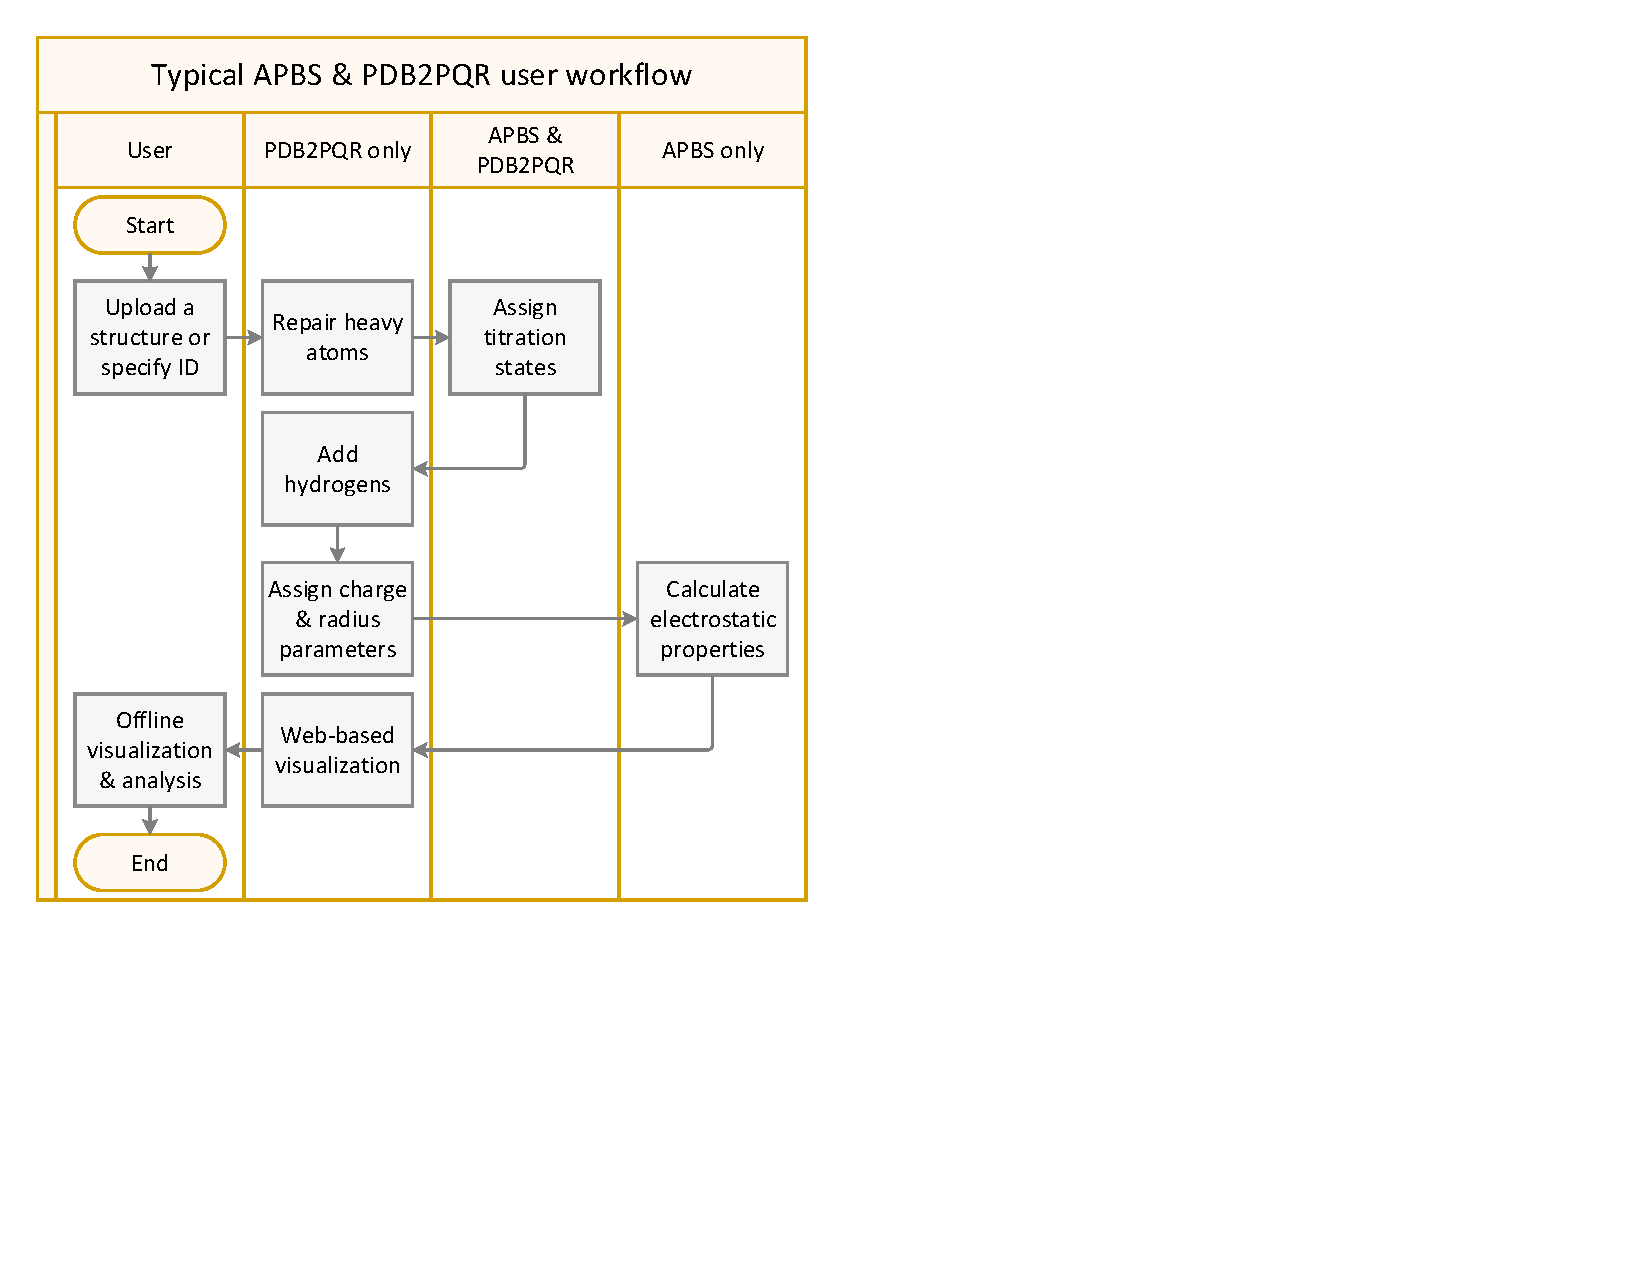
\includegraphics[width=0.60\linewidth]{APBS-and-PDB2PQR-user-flow} 
	\caption{Workflow for biomolecular electrostatics calculations using the APBS software suite.}
	\label{fig:PDB2PQR-APBS}
\end{figure}
%%%
In particular, PDB2PQR automatically sets up, executes, and optimizes the structure for Poisson-Boltzmann electrostatics calculations, outputting a PQR file that can be used with APBS or other modeling software.
Some of the key steps in PDB2PQR are described below.

\paragraph{Repairing missing heavy atoms.}
Within PDB2PQR, the PDB file is examined to see if there are missing heavy (non-hydrogen) atoms.
Missing heavy atoms can be rebuilt using standard amino acid topologies in conjunction with existing atomic coordinates to determine new positions for the missing heavy atoms.
A \textit{debump} option performs very limited minimization of sidechain $\chi$ angles to reduce steric clashes between rebuilt and existing atoms.

\paragraph{Optimizing titration states}
Amino acid titration states are important determinants of biomolecular (particularly enzymatic) function and can be used to assess functional activity and identify active sites. The APBS-PDB2PQR system contains several methods for this analysis.
\begin{itemize}
	\item \textit{Empirical methods.}
	PDB2PQR provides an empirical model (PROPKA \cite{Sondergaard2011}) which uses a heuristic method to compute p$K_a$ perturbations due to desolvation, hydrogen bonding, and charge-charge interactions is included in PDB2PQR.
	The empirical PROPKA method has surprising accuracy for fast evaluation of protein p$K_a$ values \cite{Li2005}.
	\item \textit{Implicit solvent methods.}
	PDB2PQR also contains two methods for using implicit solvent (Poisson-Boltzmann) models for predicting residue titration states.
	The first method uses Metropolis Monte Carlo to calculating titration curves and p$K_a$ values (PDB2PKA); however, sampling issues can be a major problem with Monte Carlo methods when searching over the $\mathcal{O}\left(2^N\right)$ titration states of $N$ titratable residues.
	The second method is a new polynomial-time algorithm for the optimization of discrete states in macromolecular systems \cite{Purvine2016}.
	This method transforms interaction energies between titratable groups into a graphical flow network.
	The polynomial-time $\mathcal{O}\left(N^4\right)$ behavior makes it possible to rigorously evaluate titration states for much larger proteins than Monte Carlo methods.
\end{itemize}

\paragraph{Adding missing hydrogens.}
The majority of PDB entries do not include hydrogen positions.
Given a titration state assignment, PDB2PQR uses Monte Carlo sampling to position hydrogen atoms and optimize the global hydrogen-bonding network in the structure \cite{Nielsen2001}.
Newly added hydrogen atoms are checked for steric conflicts and optimized via the debumping procedure discussed above.

\paragraph{Assigning charge and radius parameters}
Given the titration state, atomic charges (for $\rho$) and radii (for $\epsilon$ and $V_i$) are assigned based on the chosen force field.
PDB2PQR currently supports \todo{list force fields}.

\section{Solving the Poisson-Boltzmann equation}
Several software packages have been developed to analyze the solvation properties of small and macro-molecules, solving the Poisson-Boltzmann equations to evaluate energies, potentials, and other solvation properties.
The most significant (based on user base and citations) of these include CHARMM \cite{Brooks2009}, AMBER \cite{Case2005}, DelPhi \cite{Sarkar2013}, Jaguar \cite{Bochevarov2013}, Zap \cite{Grant2001}, MIBPB \cite{Chen2011}, and APBS \cite{APBS}.
The CHARMM and AMBER packages are multipurpose software designed for a wide range of modeling tasks while DelPhi and MIBPB are the most similar to APBS.
Like APBS, DelPhi has a significant and established user base; MIBPB is a newer package.
At the time of writing this manuscript, APBS had over 27,000 registered users.

The APBS software was designed from the ground up using modern design principles to ensure its ability to interface with other computational packages and evolve as methods and applications change over time.
As described in the remainder of this section, APBS provides several different methods for solving the Poisson-Boltzmann equation.

\subsection{Finite difference and finite element solvers}
The original version of APBS was based on two key libraries from the Holst research group.
FEtk (\url{http://www.fetk.org/}) is a general-purpose multi-level adaptive finite element library \cite{FEtk}.
Adaptive finite element methods can resolve extremely fine features of a complex system (like biomolecules) while solving the associated equations over large problem domain.
For example, FEtk has been used to solve electrostatic and diffusion equations over six orders of magnitude in length scale \cite{Tai}.
\cite{PMG} to solve the Poisson-Boltzmann equation.
The finite difference PMG solver trades speed and efficiency for the high-accuracy and high-detail solutions of the finite element FEtk library.
However, many APBS users need only a relatively coarse-grained solution of $\phi$ for their visualization or simulation applications.
Therefore, most APBS users employ the Holst group's finite difference grid-based PMG solver for biomolecular electrostatics calculations.

\todo{STOPPED HERE}

\subsection{Boundary element methods}
In order to address some of the issues with the numerical methods in APBS, a treecode accelerated boundary integral PB solver (TABI-PB) developed by Geng and Krasny \cite{geng2013} has recently been implement. This method provides a boundary element approach to the linearized PB equation. In this method, two coupled integral equations defined on the solute-solvent boundary define a mathematical relationship between the electrostatic surface potential $\phi_1$ and its normal derivative with a set of integral kernels consisting of Coulomb and screened Coulomb potentials with their normal derivatives. The method requires a surface triangulation, generated by a program such as MSMS \cite{sanner1995} or NanoShaper \cite{decherchi2013}, on which to discretize the integral equations. The resulting linear system is then solved with GMRES iteration \cite{saad1986}. To reduce the computational cost of this dense system from $O(N^2)$ to $O(N\log N)$, a Cartesian particle-cluster treecode is employed to compute matrix-vector products.

The matrix-vector products involve evaluation of the integral kernels over the surface elements. These evaluations effectively take the form of an $N$-body potential: a sum over a set of $N$ positions of products between a kernel and a "charge" at each position. In this case, the locations of the $N$ particles are the centroids of the surface triangularization elements. To rapidly evaluate the $N$-body potential at the $N$ particle locations, the treecode subdivides the particles into a tree-like hierarchical structure of clusters. At each location, the potential contribution from nearby particles is computed by direct sum, while for far particle clusters, a Taylor approximation about the center of the cluster is used to evaluate the contribution. The Taylor coefficients are calculated through recurrence relations. 

The TABI-PB method utilizes a well-posed boundary integral PB formulation to ensure rapid convergence. In addition, a fast treecode algorithm for the screened Coulomb potential \cite{Li2009} is applied to speed up the matrix-vector products in each GMRES iteration \cite{Juffer1991}. The TABI-PB solver serves as an effective alternative to the multi-grid finite difference solver when the surface potential accuracy or system memory capacity becomes a concern.

The coupled second kind integral equations employed by TABI-PB for calculating the surface potential $\phi_1$ and its normal derivative \cite{Juffer1991}, are as follows: 
%
\begin{equation}\label{eq:integraleq}
\begin{split}
\frac{1}{2}\left(1+\varepsilon\right)\phi_1\left({\bf x}\right) =& \int_\Gamma\left[K_1\left({\bf x}, {\bf y}\right) \frac{\partial \phi_1\left({\bf y}\right)}{\partial \nu} + K_2\left({\bf x}, {\bf y}\right) \phi_1\left({\bf y}\right) \right]dS_{\bf y} + S_1({\bf x}), \ {\bf x} \in \Gamma, \\ %
\frac{1}{2}\left(1+\frac{1}{\varepsilon}\right) \frac{\partial \phi_1\left({\bf x}\right)}{\partial \nu} =& \int_\Gamma\left[K_3\left({\bf x}, {\bf y}\right) \frac{\partial \phi_1\left({\bf y}\right)}{\partial \nu} + K_4\left({\bf x}, {\bf y}\right) \phi_1\left({\bf y}\right) \right]dS_{\bf y} + S_2({\bf x}), \ {\bf x} \in \Gamma 
\end{split} \end{equation} 
%
where $\varepsilon = \varepsilon_m / \varepsilon_s$, the ratio of the dielectric constant in the solute region and the dielectric constant in the solvent region. The integral kernels $K_1, K_2, K_3, K_4$ are defined in Eq. \ref{eq:kernels}.
%
\begin{equation}
\begin{split}
K_1\left({\bf x}, {\bf y}\right) = G_0\left({\bf x}, {\bf y}\right) - G_\kappa\left({\bf x}, {\bf y}\right),& \ \ K_2\left({\bf x}, {\bf y}\right) = \varepsilon \frac{\partial G_\kappa\left({\bf x}, {\bf y}\right)}{\partial \nu_{\bf y}}
-\frac{\partial G_0\left({\bf x}, {\bf y}\right)}{\partial \nu_{\bf y}} \\ K_3\left({\bf x}, {\bf y}\right) = \varepsilon \frac{\partial G_0\left({\bf x}, {\bf y}\right)}{\partial \nu_{\bf x}}
-\frac{1}{\varepsilon}\frac{\partial G_\kappa\left({\bf x}, {\bf y}\right)}{\partial \nu_{\bf x}},& \ \ K_4\left({\bf x}, {\bf y}\right) = \varepsilon \frac{\partial^2 G_\kappa\left({\bf x}, {\bf y}\right)}{\partial \nu_{\bf x} \partial \nu_{\bf y}}
-\frac{1}{\varepsilon}\frac{\partial^2 G_0\left({\bf x}, {\bf y}\right)}{\partial \nu_{\bf x} \partial \nu_{\bf x}}
\label{eq:kernels}
\end{split} \end{equation}
%
where $G_0$ and $G_\kappa$ are the Coulomb and screened Coulomb potentials defined as:
%
\begin{equation}
G_0\left({\bf x}, {\bf y}\right) = \frac{1}{4\pi \left|{\bf x} - {\bf y}\right|}, \ \ G_\kappa\left({\bf x}, {\bf y}\right) = \frac{e^{-\kappa\left|{\bf x} - {\bf y}\right|}}{4\pi \left|{\bf x} - {\bf y}\right|} 
\end{equation}
%
The normal derivatives of the potential kernels $G$ are:
%
\begin{equation}
\begin{split}
\frac{\partial G\left({\bf x}, {\bf y}\right)}{\partial \nu_{\bf y}} =& \sum\limits_{n=1}^{3} \nu_n\left({\bf y}\right)\partial_{y_n}G\left({\bf x}, {\bf y}\right), \\
\frac{\partial G\left({\bf x}, {\bf y}\right)}{\partial \nu_{\bf x}} =& -\sum\limits_{n=1}^{3} \nu_n\left({\bf y}\right)\partial_{x_n}G\left({\bf x}, {\bf y}\right), \\
\frac{\partial^2 G\left({\bf x}, {\bf y}\right)}{\partial \nu_{\bf x}\partial \nu_{\bf y}} =& -\sum\limits_{m=1}^{3}\sum\limits_{n=1}^{3} \nu_m\left({\bf x}\right)\nu_n\left({\bf y}\right)\partial_{x_n}\partial_{y_n}G\left({\bf x}, {\bf y}\right) 
\end{split} \end{equation}
%
for the three spatial components $n$ of the normal direction. Additionally, the source terms $S_1$ and $S_2$ in Eq. \ref{eq:integraleq} are:
%
\begin{equation}
S_1({\bf x}) = \frac{1}{\varepsilon_m}\sum\limits_{k=1}^{N_c}q_k G_0\left({\bf x}, {\bf y}_k\right), \ \ S_2({\bf x}) = \frac{1}{\varepsilon_m}\sum\limits_{k=1}^{N_c}q_k \frac{\partial G_0\left({\bf x}, {\bf y}_k\right)}{\partial \nu_{\bf x}}
\end{equation}
%
where $N_c$ is the number of atoms in the solute molecule, and $q_k$ is the charge of the $k$th atom. Note that $S_1$ is a linear superposition of the point charge electrostatic potentials, and $S_2$ is a linear superposition of the normal derivatives of the potentials.

Given a surface triangularization with $N$ elements, where ${\bf x}_i$ and $A_i$ are the centroid and area, respectively, of the $i$th triangle, the integral equations are discretized as:
%
\begin{equation}
\begin{split}
\frac{1}{2}\left(1+\varepsilon\right)\phi_1\left({\bf x}_i\right) =& \sum_{\substack{j=1 \\ j\neq i}}^N \left[K_1\left({\bf x}_i, {\bf x}_j\right) \frac{\partial \phi_1\left({\bf x}_j\right)}{\partial \nu} + K_2\left({\bf x}_i, {\bf x}_j\right) \phi_1\left({\bf x}_j\right) \right]A_j + S_1({\bf x}_i), \\ %
\frac{1}{2}\left(1+\frac{1}{\varepsilon}\right) \frac{\partial \phi_1\left({\bf x}_i\right)}{\partial \nu} =& \sum_{\substack{j=1 \\ j\neq i}}^N \left[K_3\left({\bf x}_i, {\bf x}_j\right) \frac{\partial \phi_1\left({\bf x}_j\right)}{\partial \nu} + K_4\left({\bf x}_i, {\bf x}_j\right) \phi_1\left({\bf x}_j\right) \right]A_J + S_2({\bf x}_I)
\end{split}
\end{equation}
%
The omission of the $j=i$ term in the summation avoids the singularity of the kernels at that point. Note that the right hand sides of these equations consist of sums of products of kernels and the surface potential or its normal derivative. These are the analogues to the $N$-body potential in the treecode, with the surface potential or its normal derivatives playing the role of the charges. In the discretized form, the total electrostatic energy of solvation is given by Eq. \ref{eq:tabi_TEE}.
%
\begin{equation}
E_\text{sol}=\frac{1}{2}\sum_{k=1}^{N_c}q_k\sum_{j=1}^N \left[K_1\left({\bf x}_k, {\bf x}_j\right) \frac{\partial \phi_1\left({\bf x}_j\right)}{\partial \nu} + K_2\left({\bf x}_k, {\bf x}_j\right) \phi_1\left({\bf x}_j\right) \right]A_j
\label{eq:tabi_TEE}
\end{equation}
%
where $q_k$ is the charge on the $k$th atom of the solute molecule, and ${\bf x}_k$ is its position.

Several unique features of the boundary integral formulation are worth mentioning. Because the integral equations are defined on the molecular boundary, the singular charges are handled analytically and do not introduce the same issues present in grid-based schemes. The integral equations also rigorously enforce the interface conditions on the surface, and the boundary condition at infinity is exactly satisfied. Thus, the boundary integral formulation can potentially be superior to other methods for investigating electrostatic potential on the boundary. However, because the method is only well defined for the linearized PB equation, it may perform poorly for high salt concentration in the solvent.

\paragraph{Usage in APBS}
The APBS user can invoke TABI-PB with the \texttt{bem-manual} flag in the ELEC section of the input file. TABI-PB will produce output including the potential and normal derivative of potential for every element and vertex of the triangularization, as well as the electrostatic solvation energy. The user can additionally specify the order of the Taylor expansions used in the far field potential contribution approximations, the maximum number of particles allowable in a leaf (clusters in the last level of the tree), and the multipole acceptance criterion, which determines the distance at which potential contributions from particles in a cluster are evaluated directly or through the Taylor expansion (see Table \ref{tab:TABIPB-keywords}). 

In general, a lower multipole acceptance criterion ($\theta$) will result in a more accurate but more expensive computation; a lower $\theta$ causes more direct summations and forces the particle-cluster interaction to descend to a finer cluster level. Similarly, a higher Taylor expansion order will also result in a more accurate but more expensive computation. A typical first-pass choice for these parameters would be a multipole acceptance criterion of 0.8, a Taylor expansion order of 3, and a maximum leaf size of 500. More investigation is needed to determine optimal parameter choices.

\begin{table}[!htbp]
	\begin{minipage}{0.99\textwidth}
		%\vspace{-12pt}
		\centering
		\caption{\small Keywords used in TABI-PB. For more details and examples of implementation, please see the APBS website. }
		\vspace{1mm}
		
		\newcommand{\param}[1]{\textless\texttt{#1}\textgreater}
		\newcommand\T{\rule{0pt}{0.8ex}}       % Top strut
		
		%\newlength{\colthree}
		\setlength{\colthree}{8.3cm}
		%\newlength{\coltwo}
		\setlength{\coltwo}{2.8cm}
		{\small
			\begin{tabular}{ l  l l  }				
				{Keyword} & {Parameters} & {Description} \\ \hline
				\T tree\_order & \param{order} & \parbox[t]{\colthree}{Integer indicating the order of the Taylor expansion for determining treecode coefficients.} \\
				\T tree\_n0 & \param{max\_number} & \parbox[t]{\colthree}{Maximum number of particles allowable in a treecode leaf.}\\ 
				\T mac & \param{theta} & \parbox[t]{\colthree}{Multipole acceptance criterion, specifies the distance ratio at which the Taylor expansion is used.}\\ 
				\hline 
				\T mesh & \param{flag} & \parbox[t]{\colthree}{Software to be used for meshing the molecular surface: 0=MSMS, 1=NanoShaper's SES implementation, and 2=NanoShaper's Skin implementation.}  \\
				\hline
				\T outdata & \param{flag} & \parbox[t]{\colthree}{Type of output data file generated: 0=APBS format and 1=compatible with ParaView (including VTK data file).}  \\
				\label{tab:TABIPB-keywords}
			\end{tabular}
		} % end small
	\end{minipage}
\end{table}
%\vspace{-5pt}
%
The user can also choose to specify whether TABI-PB uses MSMS, the SES implementation in NanoShaper, or the Skin surface implementation of NanoShaper to generate a surface triangularization, as shown in Figure \ref{fig:surface-mesher}. NanoShaper, an open-source program for surface triangularization, was recently added to TABI-PB, and preliminary results suggest superior performance to MSMS. Examples of surface potential on 1a63 are given in Figure \ref{fig:surface-protential} by using MSMS and NanoShaper.
%
\begin{figure}[h!]
	%\vspace{-60pt}
	\vspace{-10pt}
	\centering
	\hspace{-5pt}
	(A)~\hspace{-3pt}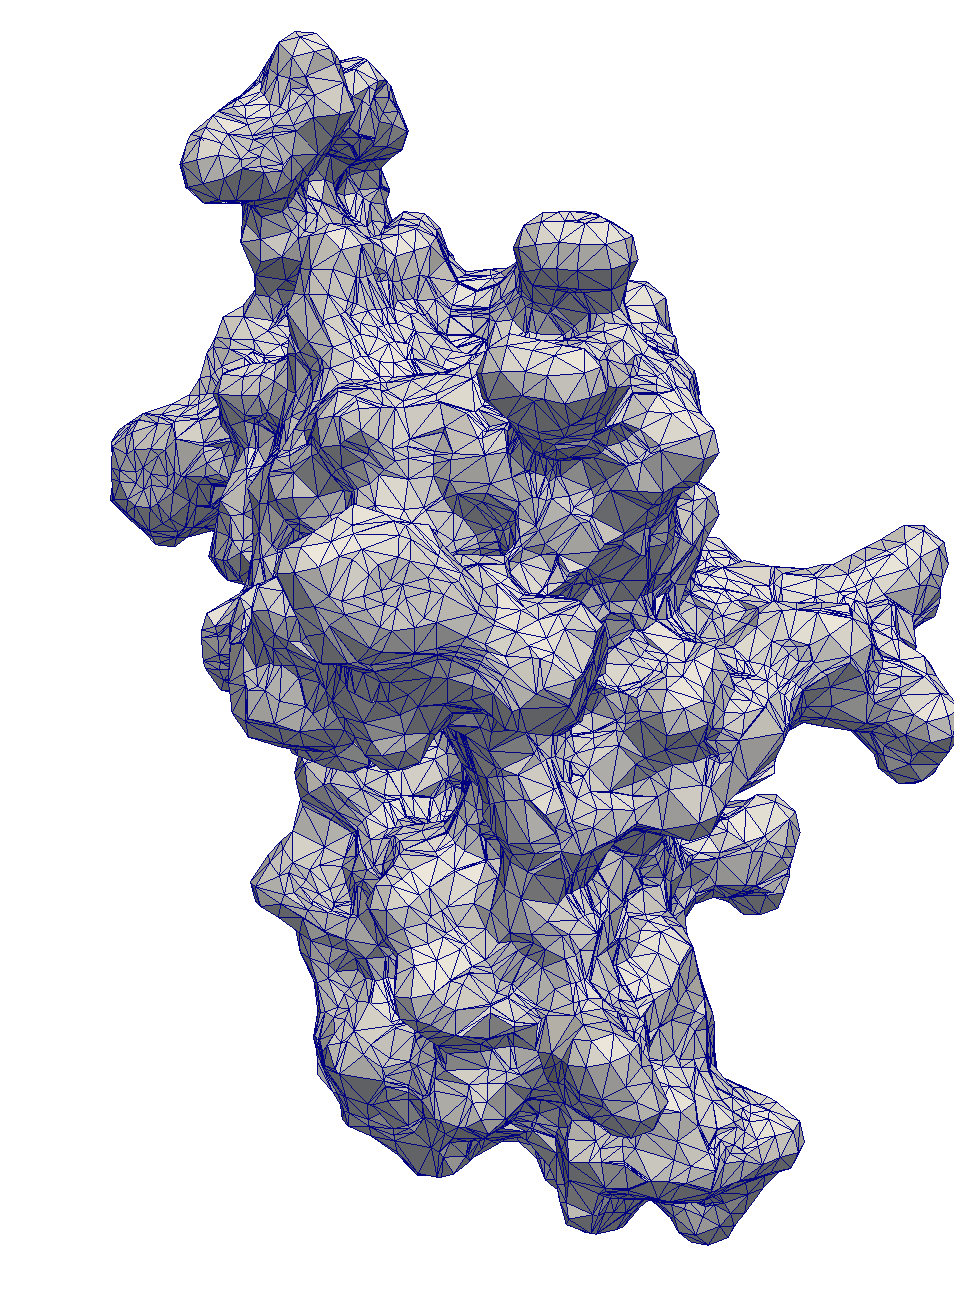
\includegraphics[width=0.25\linewidth]{msmsSEStriangwire.png} 
	\hspace{-10pt}
	(B)~\hspace{-3pt}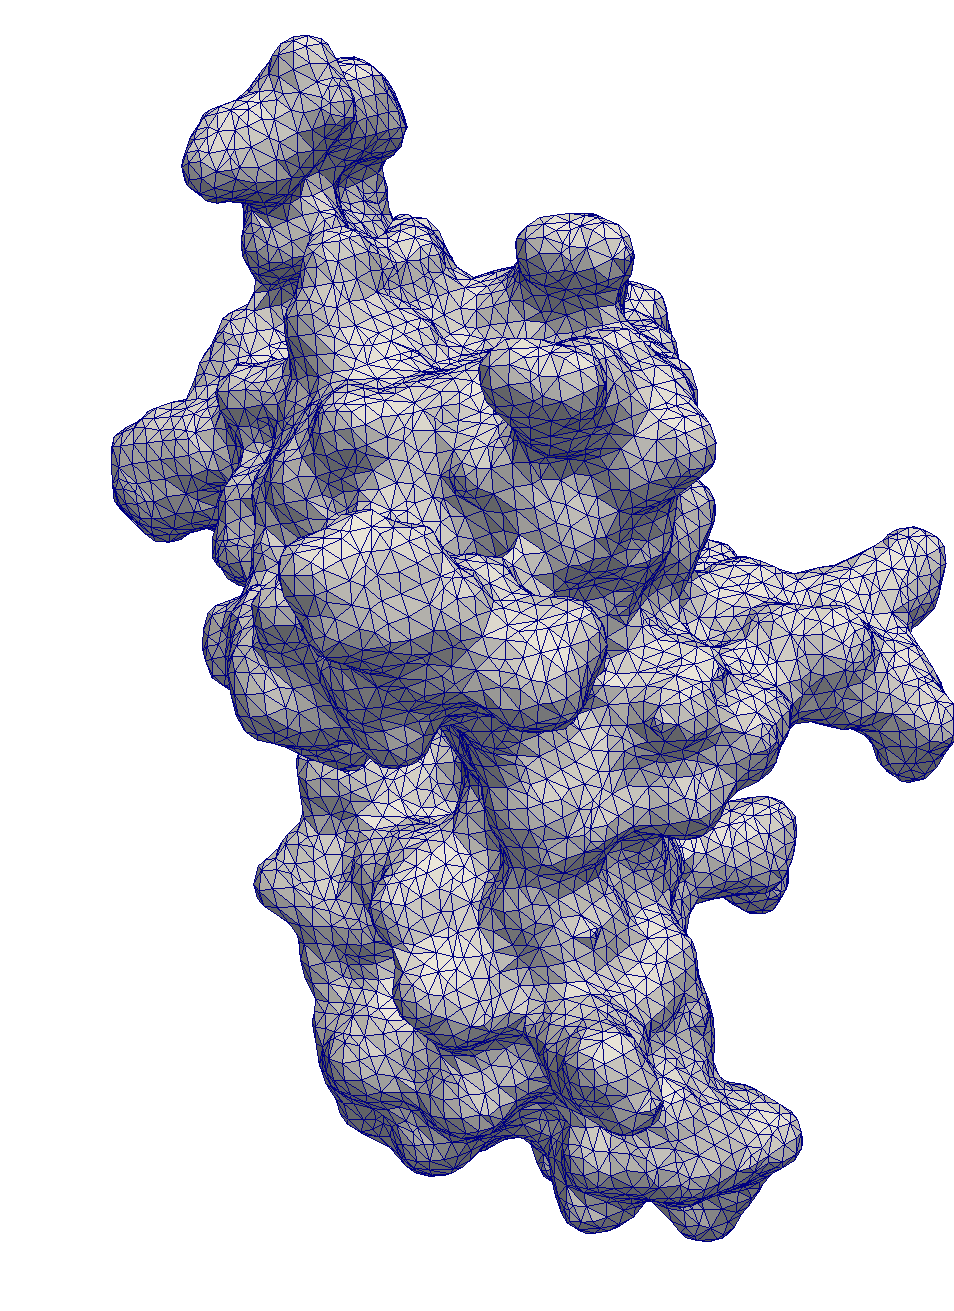
\includegraphics[width=0.25\linewidth]{NSSEStriangwire.png}
	\hspace{-10pt} 
	(C)~\hspace{-3pt}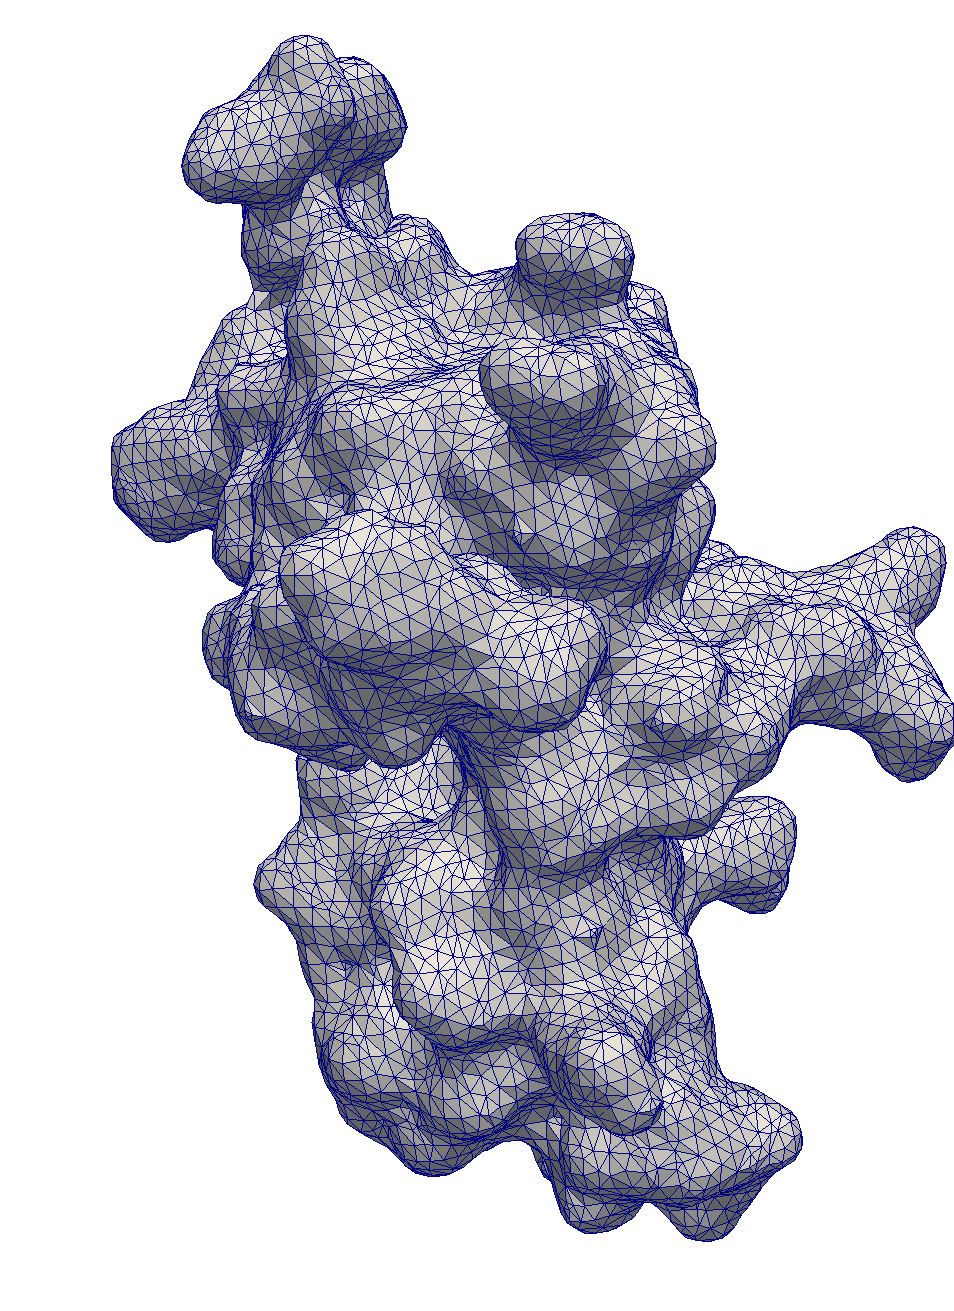
\includegraphics[width=0.25\linewidth]{NSSkintriangwire.png}
	\hspace{-5pt}
	%\vspace{-10pt}
	\caption{\small PDB ID 1a63 surfaces generated with 
		(A) MSMS, number of triangles=20228;
		(B) NanoShaper SES, number of triangles=20744;
		(C) NanoShaper Skin, number of triangles=21084.}
	\label{fig:surface-mesher}
	%\vspace{-1em}
\end{figure}
%
\begin{figure}[h!]
	\vspace{-10pt}
	\centering
	\hspace{-5pt}
	(A)~\hspace{-3pt}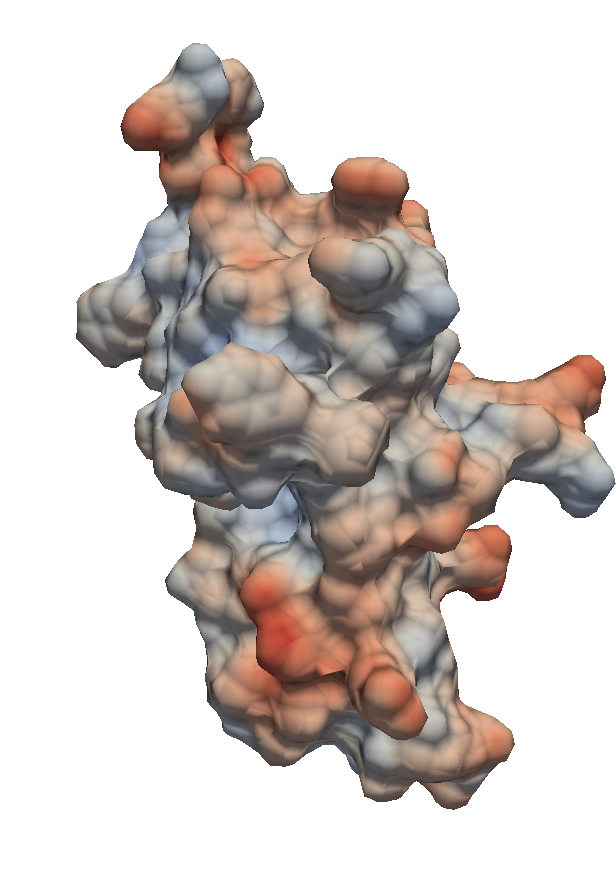
\includegraphics[angle=0,width=0.25\linewidth]{msmsSES.png} 
	\hspace{-10pt}
	(B)~\hspace{-3pt}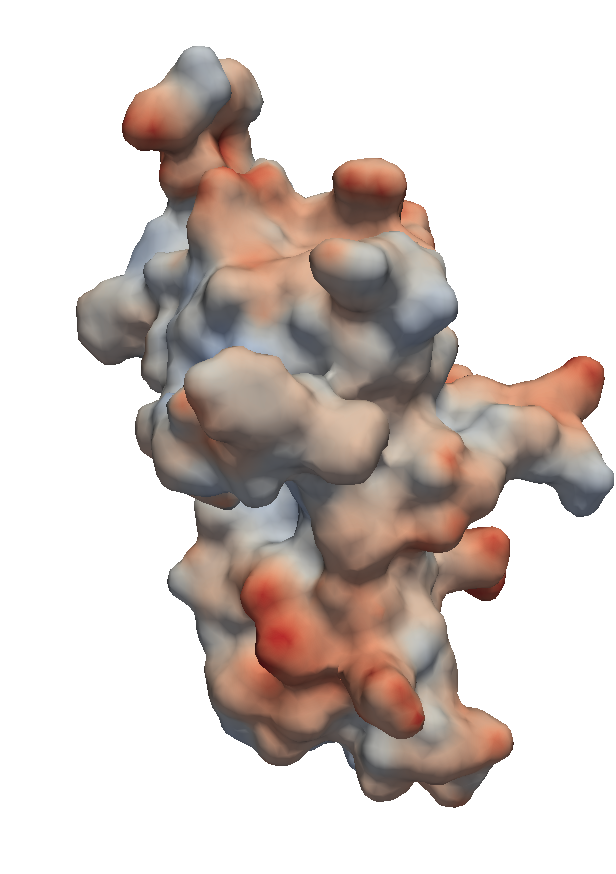
\includegraphics[angle=0,width=0.25\linewidth]{NSSES.png}
	\hspace{-10pt} 
	(C)~\hspace{-3pt}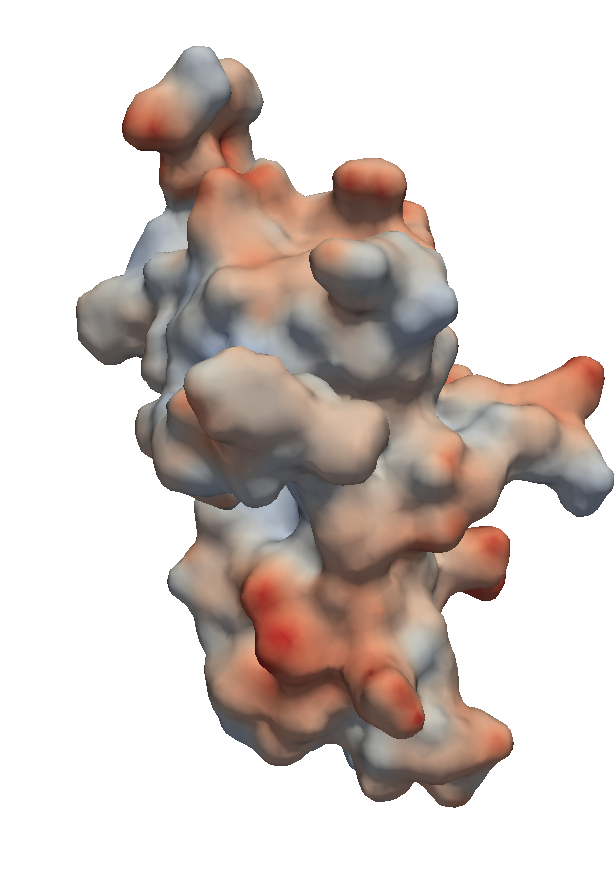
\includegraphics[angle=0,width=0.25\linewidth]{NSSkin.png}
	\hspace{-5pt}
	%\vspace{-10pt}
	\caption{\small 1a63 visualization of surface potential for
		(A) MSMS, max=5.06 kcal/mol, min=-5.15 kcal/mol;
		(B) NanoShaper SES, max=4.44 kcal/mol, min=-7.95 kcal/mol;
		(C) NanoShaper Skin, max=4.25 kcal/mol, min=-20.03 kcal/mol.}
	\label{fig:surface-protential}
	\vspace{-1em}
\end{figure}

\subsection{Analytical and semi-analytical methods}
As mentioned above, numerical solution methods tend to be computationally intensive. Therefore, analytical methods have been included in the APBS system, which is beneficial for a rapid and accurate solution of the PB equation.

\paragraph{Poisson-Boltzmann Analytical Method}
The Poisson-Boltzmann Analytical Method (PB-AM), was developed by Lotan and Head-Gordon in 2006 \cite{lotan2006}. It presents a fully analytical solution to the linearized PB equation for multiple macromolecules in a screened environment. Each molecule in the system is coarse-grained and represented as a single low dielectric spherical cavity. This domain enables the use of the multipole expansion to represent charge-charge interactions and higher order cavity polarization effects. The solution to this model is represented as a system of linear equations as follows:
%
\begin{equation}\label{eq:pbam_solve}
\mathbf{A} = \Gamma \cdot (\Delta \cdot T \cdot \mathbf{A} + \mathbf{E})
\end{equation}
%
Where \(\mathbf{A}\) represents a vector of the effective multipole expansion of the charge distributions of each molecule, \(\mathbf{E}\) is a vector of the fixed charge distribution of all molecules, \(\Gamma\) is a dielectric boundary-crossing operator, \(\Delta\) is a cavity polarization operator and \(T\) is an operator that transforms the multipole expansion from the global (lab) coordinates to a local coordinate frame. Once the unknown \textbf{A}'s are solved using the Gauss-Sieidel iterative method, many physical properties, such as interaction energies, forces and torques can be computed. The interaction energy for molecule \(i\), ($\Omega^{(i)}$) is given in Eq. \ref{eq:pbam_energy}.
%
\begin{equation}\label{eq:pbam_energy}
\Omega^{(i)}=\frac{1}{\epsilon_s} \left \langle \sum_{j \ne i}^N  T \cdot A^{(j) } ,  A^{(i) } \right \rangle 
\end{equation}
%
where $\epsilon_s$ is the dielectric constant of the solvent and $\langle  M, N \rangle$ denotes the inner product. When energy is computed, forces follow as:
%
\begin{equation}\label{eq:pbam_force}
\textbf{F}^{(i)} = \nabla_i \Omega^{(i)}=\frac{1}{\epsilon_s} [ \langle \nabla_i \,T \cdot A^{(i) } ,  A^{(i) } \rangle +  \langle T \cdot A^{(i) } ,   \nabla_i \, A^{(i) } \rangle ]
\end{equation}
%
By definition, the torque on a charge in the molecule is the cross product of its position relative to the center of mass of the molecule with the force it experiences. The total torque on the molecule is a linear combination of the torque on all charges of the molecule, as illustrated in Eq. \ref{eq:pbamtor}.
%
\begin{equation}\label{eq:pbamtor}
\tau^{(i)} =  \frac{1}{\epsilon_s}\left [  ^xH^{(i)}, ^yH^{(i)}, ^zH^{(i)} \right] \times   \left [  \nabla_i L^{(i)} \right ]
\end{equation} 
%
where $^\alpha H_{n,m}^{(i)}  = \sum_{j=1}^{M_i} \alpha_{j}^{(i)} \gamma_n^{(i)} q_j^{(i)} (\rho_j^{(i)})^n Y_{n,m} (\vartheta_j^{(i)}, \varphi_j^{(i)}) \, , \, \alpha = x , y, z$, is a coefficient vector for each of the charges in the molecule, $M_i$ is the number of charges in molecule $i$, $q_J^{(i)}$ is the magnitude of the $j^{th}$ charge, and $p_j^{(i)}=\Big[\rho_j^{(i)},\vartheta_j^{(i)},\varphi_j^{(i)}\Big]$ is its position in spherical coordinates. For more details on the PB-AM derivation, see Lotan, Head-Gordon \cite{lotan2006}.

\paragraph{Poisson Boltzmann Semi-Analytical Method}

An extension of the fully analytical solution, the Poisson Boltzmann Semi-Analytical method (PB-SAM) incorporates the use of boundary integrals into its formalism to represent a complex molecular domain as a collection of overlapping low dielectric spherical cavities \cite{yap2010}.  It presents a semi-analytical solution to the linearized PB equation for multiple macromolecules in a screened environment. The semi-analytical method provides a better representation of the molecular boundary when compared to PB-AM, while maintaining computational efficiency.

Because it is fully analytical, PB-AM can be used for model validation as well as for representing systems that are relatively spherical in nature, such as globular proteins and colloids. PB-SAM, on the other hand has a much more detailed representation of the molecular surface and can therefore be used for many systems that other APBS (numerical) methods are currently used for. Additionally, both methods have been implemented in a Brownian dynamics (BD) scheme \cite{ermak1978} and can perform dynamics with full mutual polarization, a novel feature for APBS.

The derivation details of PB-SAM have been reported  previously \cite{yap2010,yap2013}, with the main points being summarized in this section. The electrostatic potential ($\phi_r$) of the system at any point $r$ is governed by the linearized form of the PB equation:

\begin{equation}
\nabla \cdot [ \epsilon(\mathbf{r}) \nabla \phi (\mathbf{r}) ] - \epsilon (\mathbf{r}) \kappa^2 \phi(\mathbf{r}) = 4 \pi \rho(\mathbf{r})
\label{eq:pbsam_lpbe}
\end{equation}
%
where $\kappa$ is the inverse Debye length. For the case of spherical cavities, we can solve Eq. \ref{eq:pbsam_lpbe} by dividing the system into inner sphere and outer sphere regions, and enforcing a set of boundary conditions that stipulate the continuity of the electrostatic potential and the electrostatic field at the surface of each sphere. The electrostatic potential outside molecule ($I$) is described by:
%
\begin{equation}
\phi_{out}^{(i)} (\mathbf{r})  = \sum_{I=1}^{N_{mol}} \left( 4 \pi \int_{d\Omega^{(I)}} \frac{e^{-\kappa | r - r'|}}{|r - r'|} h^{(I)} (r') dr'  \right)
\label{eq:pbsam_phi_in}
\end{equation}
%
where \(h(r)\) is an effective surface charge that can be transformed into the unknown multipole expansion \(H^{(I,k)}\) with inside molecule \textit{I} and sphere \textit{k}. In a similar manner, the interior potential is given as
%
\begin{equation}
\phi_{in}^{(i)} (\mathbf{r})  = \sum_{\alpha = 1}^{N_C^{(I)}} \frac{1}{|r-r_{\alpha}^{(I)}|} \cdot \frac{q_\alpha^{(I)}} {\epsilon_{in}} + \frac{1}{4\pi} \int_{d\Omega^{(I)}} \frac{1}{|r - r'|} f^{(I)} (r') dr' 
\label{eq:pbsam_phi_out}
\end{equation}
%
where \( N_C^{(I)}\) is the number of charges in molecule \textit{I}, \( q_\alpha\) 
is the magnitude of the \(\alpha\)-th charge, \( r_\alpha^{(I)} = \Big[\rho_{\alpha}^{(I)} , \theta_{\alpha}^{(I)} , \phi_{\alpha}^{(I)} \Big]\) is its position in spherical 
coordinates, and \(f(r)\) is a reactive surface charge that can
be transformed into the unknown multipole expansion \(F^{(I,k)}\). The reactive multipole and the effective multipole, \(H^{(I,k)}\), are given as:
%
\begin{equation}
F_{n,m}^{(I,k)} \equiv  \frac{1}{4\pi} \int_{d\Omega^{(I,k)}} f^{(I,k)}(r') \left (  \frac{ a^{(I,k)}}  {r'} \right ) ^{n+1} \overline{ Y^{(I,k)}_{n,m}} (\theta' , \phi') dr'
\label{eq:fmat}
\end{equation}
%
\begin{equation}
H_{n,m}^{(I,k)} \equiv  \frac{1}{4\pi} \int_{d\Omega^{(I,k)}} h^{(I,k)}(r') \left (  \frac{ r'}{a^{(I,k)}} \right ) ^{n} \hat{i}_n(\kappa r') \overline{ Y^{(I,k)}_{n,m}} (\theta' , \phi') dr'
\label{eq:hmat}
\end{equation}
%
where \(Y_{n,m}\) is the spherical harmonics, $\overline{Y_{n,m}}$ is the complete conjugate, and \(a^{(I,k)}\) is the radius of sphere \textit{k} of molecule \textit{I}. These multipole expansions can be iteratively solved using:
%
\begin{equation}
F_{n,m}^{(I,k)} = \langle I_{E, n,m} ^{(I,k)}, WF^{(I,k)} \rangle
\label{eq:fmat_it}
\end{equation}
%
\begin{equation}
H_{n,m}^{(I,k)} = \langle I_{E, n,m} ^{(I,k)}, WH^{(I,k)} \rangle
\label{eq:hmat_it}
\end{equation}
%
where $WF^{(I,k)}$ and $WH^{(I,k)}$ are scaled multipoles computed from fixed charges and polarization charges from other spheres. \(I_{E,n,m}^{(I,k)}\) is a matrix of the surface integrals over the exposed surface:
%
\begin{equation}
I_{E, n,m} ^{(I,k)} \equiv \frac{1}{4\pi } \int_{\phi_E} \int_{\theta_E} Y_{l,s}^{(I,k)}  (\theta', \phi') \overline{Y_{n,m}^{(I,k)}} (\theta', \phi') sin \theta' d\theta' d \phi' 
\label{eq:imat}
\end{equation}
%
Using the above formalism, physical properties of the system, such as interaction energy, forces and torques may be computed. The interaction energy of each molecule, ($\Omega^{(i)}$), is the product of the molecule's total charge distribution (from fixed and polarization charges) with the potential due to external sources. This is computed as the inner product between the molecule's multipole expansion, ($H^{(I,k)}$), and the multipole expansions of the other molecules in the system, ($LHN^{(I,k)}$) as follows:
%
\begin{equation}
\Omega^{(i)} = \frac{1}{\epsilon_s} \sum_{k}^{N_k^{(I)}}  \langle LHN^{(I,k)}, H^{(I,k)} \rangle
\label{eq:pbsam_en_interact}
\end{equation}
%
which allows us to define the force which is computed as the gradient of the interaction energy with respect to the position of the center of molecule \textit{I}:

\begin{equation}
F^{(I)} = - \nabla \Omega^{(I)} =  -  \frac{1}{\epsilon_s} \sum_{k}^{N_k^{(I)}} f_{I,k} = -  \frac{1}{\epsilon_s} \sum_{k}^{N_k^{(I)}}( \langle \nabla LHN^{(I,k)}, H^{(I,k)} \rangle +  \langle LHN^{(I,k)}, \nabla H^{(I,k)} \rangle)
\label{eq:pbsam_force}
\end{equation}
%
As in the analytical method, the torque on a charge in the molecule is the cross product of its position relative to the center of mass of the molecule with the force it experiences. For a charge at position, \(P\), about the center of mass \(c^{(I)}\) for molecule \(I\), the torque is given by the cross product of its position, \(r_P^{(I,k)}\), with respect to the center of mass and the force on that charge, $f_P$. We can re-express \(r_P^{(I,k)}\) as the sum of vectors from the center of molecule $I$ to the center of sphere \(k\) (\(c^{(I,k)}\)) and from the center of sphere \(k\) to point $P$ \((r_P^{(I,k)})\). The total torque on molecule \(I\) is then given by Eq. \ref{eq:pbsam_torque}.
%
\begin{equation}
\tau^{(I)} =  \sum_{k}^{N_k^{(I)}} c^{(I,k)} \times   f_{I,k} + \sum_{k}^{N_k^{(I)}}  \sum_{P\in k} r_P^{(I,k)} \times f_P 
\label{eq:pbsam_torque}
\end{equation}
%
where \(f_{I,k}\) is given in Eq. \ref{eq:pbsam_force} and

\begin{equation}
f_P = -  \frac{1}{\epsilon_s} \sum_{k}^{N_k^{(I)}}( \langle \nabla_I LHN^{(I,k)}, H_P^{(I,k)} \rangle +  \langle LHN^{(I,k)}, \nabla_I H_P^{(I,k)} \rangle)
\label{eq:pbsam_torque_fp}
\end{equation}
%
where
\begin{equation}
H_{P,n,m}^{(I,k)} =h(\theta_p, \phi_p) Y_{n,m}^{(I,k)} (\theta_p, \phi_p) 
\label{eq:pbsam_hp}
\end{equation}
%
\begin{equation}
\nabla_j H_{P,\alpha, n,m}^{(I,k)} = \left [ \nabla_j \, h(\theta_p, \phi_p) \right ]_{\alpha}   Y_{n,m}^{(I,k)} (\theta_p, \phi_p) 
\label{eq:pbsam_derv_hp}
\end{equation}
%
where \(\alpha = x , y, z\). For the derivation of the PB-SAM solver please see the previous publications \cite{yap2010, yap2013} .

\paragraph{Usage in APBS}
PB-AM and PB-SAM have been fully integrated into APBS, and is invoked using the keyword \texttt{pbam-auto} or \texttt{pbsam-auto} in the ELEC section of an APBS input file.\footnote{www.poissonboltzmann.org/docs/apbs-overview} From APBS, both programs can be used to compute the electrostatic potential at any point in space, report energies, forces, and torques of a system of macromolecules, and simulate a system using a BD scheme \cite{ermak1978}. For an example of the key simulation commands used in a run of PB-AM or PB-SAM, see Table \ref{tab:PBsAM-keywords_abbrev}. The \texttt{term} keyword, included in Table \ref{tab:PBsAM-keywords_abbrev}, allows the user to indicate conditions for the termination of each BD trajectory. This may include the contact of two molecules or the diffusion of a specified molecule beyond a specified point in space, like the conditions defined by Northrup, Allison and McCammon for the NAM simulation protocol \cite{northrup1984}. In addition to parameters specific to each type of run (BD, electrostatic potential printing and physical calculations), the user can modify the coarseness of the molecular description by modifying the coarse-graining parameter \texttt{tolsp}, which indicates how far beyond the solvent-excluded surface the coarse-grain molecular boundary is allowed to extend. The larger the value of \texttt{tolsp}, the coarser the description of the molecule, e.g. less coarse grain spheres used to represent it. This will make computational evaluation of the system more rapid, but less accurate. Conversely, the smaller the \texttt{tolsp} value chosen, the more coarse grain spheres needed to represent the system, which means a more accurate but also more costly representation of the system. The \texttt{tolsp} parameter is generally in the range of 1 to 5 \AA. The commands (keywords) not included in Table \ref{tab:PBsAM-keywords_abbrev} are used to specify system conditions, such as temperature and salt concentration.

\begin{table}[!ht]
	\begin{minipage}{0.99\textwidth}
		%\vspace{-12pt}
		\vspace{5pt}
		\newcommand{\param}[1]{\textless\texttt{#1}\textgreater}
		\newcommand\T{\rule{0.0pt}{0.8ex}}       % Top strut
		
		\newlength{\colthree}
		\newlength{\coltwo}
		\setlength{\colthree}{8.3cm}
		\setlength{\coltwo}{2.8cm}
		
		\centering
		\caption{\small Major keywords used in PB-AM and PB-SAM. For more keywords, details and examples of implementation, please see the APBS website.}
		\vspace{1mm}
		{\small
			\begin{tabular}{ l  l l  }
				{Keyword} & {Parameters} & {Description} \\ \hline
				%    \textbf{Keyword} & \textbf{Parameters} & \textbf{Description} \B\\ \hline
				\T runname & \param{name} & \parbox[t]{\colthree}{Desired name to be used for outputs of each run.} \\
				\T pbc & \param{boxlength} & \parbox[t]{\colthree}{Size of periodic box.}\\ 
				\hline
				\T runtype dynamics & \parbox[t]{\coltwo}{ } & \parbox[t]{\colthree}{Perform a Brownian Dynamics run.}  \\ 
				\T ntraj & \parbox[t]{\coltwo}{ \param{trajct}} & \parbox[t]{\colthree}{Number of trajectories to run.}  \\ 
				\T term & \parbox[t]{\coltwo}{\param{type} \param{val} \param{mols}} & \parbox[t]{\colthree}{Attributes of a termination condition: \param{type} can be \texttt{time},  \texttt{x<=, y<=, z<=, r<=}, (or the \texttt{>=} equivalents), \param{val} is the value of the condition, \param{mols} is the molecular index that this condition applies to (\texttt{time} requires 0, all else, 1). } \\ 
				\T xyz & \parbox[t]{\coltwo}{\param{idx} \param{fpath} }& \parbox[t]{\colthree}{Molecule index and file name (path) for the xyz file. A starting configuration is needed for each trajectory for all the molecules, so there should be \param{trajct} xyz lines for each molecule. } \\ %\hline 
				
				\multicolumn{3}{c} {\textbf{PB-SAM Keywords}}  \\ \hline
				\T msms & \parbox[t]{\coltwo}{ } & \parbox[t]{\colthree}{ Will run the MSMS program for the coarse-graining process.}  \\ 
				\T tolsp & \parbox[t]{\coltwo}{ \param{tol}} & \parbox[t]{\colthree}{For the coarse-graining process, a tolerance in (\AA) to indicate how far from the molecule surface the coarse grain surface is allowed to extend. }  \\ 
				\label{tab:PBsAM-keywords_abbrev}
			\end{tabular}
		} % end small
	\end{minipage}
\end{table}
%\vspace{-5pt}

Examples of electrostatic potential (ESP) visualization results from PB-AM are given in Figure \ref{fig:pbam-results}. In Figure \ref{fig:pbam-results} (A), 2-D cross sections of electrostatic potential surrounding two spheres of opposite charge are shown. The 3-D surface potential visualization given in Figure \ref{fig:pbam-results} (B) describes the potential on the surface of a coarse-grain barstar molecule (a ribonuclease inhibitor). Figure \ref{fig:pbam-results} (C) is an example of three-dimensional isosurface visualization in VMD \cite{humphrey1996}. The molecule system which was analyzed was the periplasmic face of the Omp32 Porin trimer, a transmembrane protein. The periplasmic face (channel exit) has a positive surface (blue) at the channel exit which may further enhance anion transport through the channel.  

ESP visualization results are given in Figure \ref{fig:pbsam-results} for the PB-SAM model. They include the visualizations of barnase and barstar molecules, a ribonuclease and its inhibitor, whose association is driven by electrostatic interactions. Figure \ref{fig:pbsam-results} (A) is a two-dimensional cross section visualization of a barnase molecule. The molecule interior is given in dark blue and the color bar indicates the spatial variation of the potential with the molecule centered at the origin. Figure \ref{fig:pbsam-results} (B) is a visualization of the potential of a barstar molecule at its association interface. The positive potential distribution at the surface interacts favorably with the negative potential distribution on the barnase surface. Figure \ref{fig:pbsam-results} (C) visualizes the electrostatic potential surrounding the barnase-barstar interaction complex. 
%
\begin{figure}[th!]
	\centering
	(A)~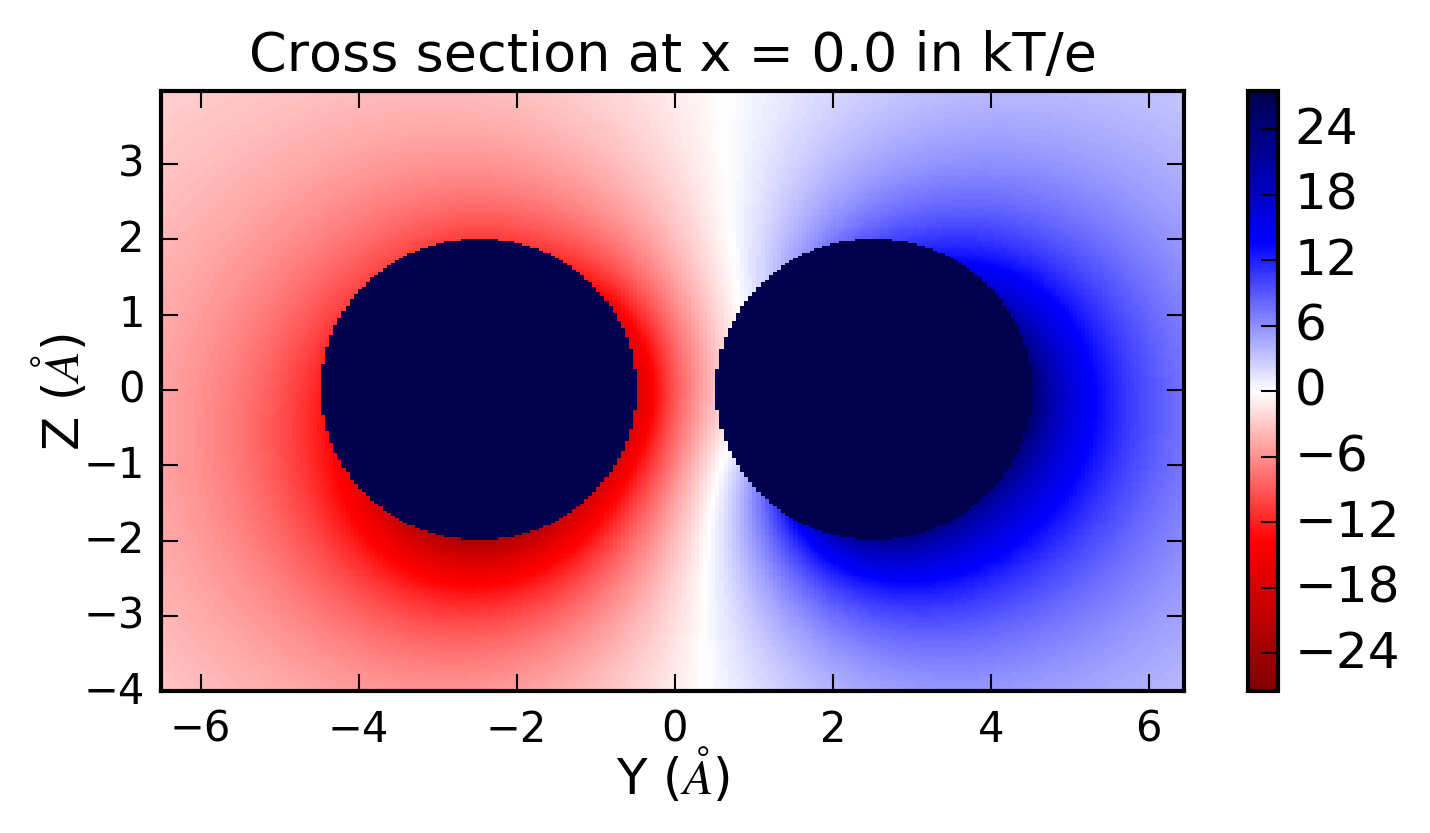
\includegraphics[width=0.40\linewidth]{pbam_toy} 
	(B)~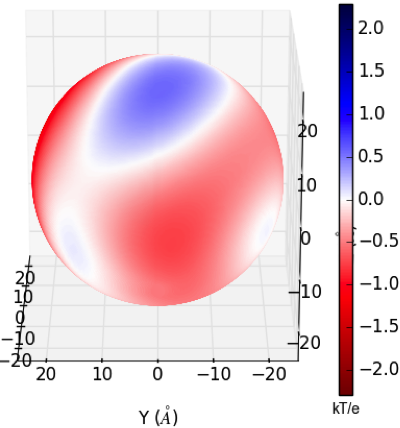
\includegraphics[width=0.23\linewidth]{pbam_barstar} 
	(C)~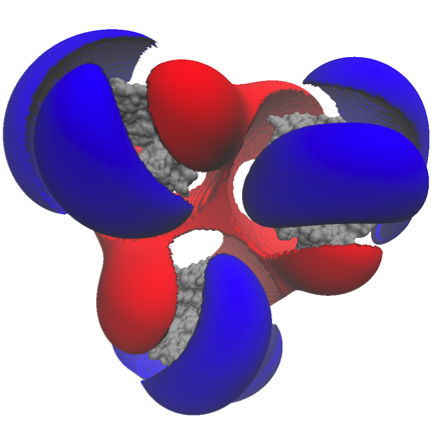
\includegraphics[width=0.23\linewidth]{pbam_porin}
	\vspace{-10pt}
	\caption{\small ESP results derived from APBS PB-AM (0.0M salt, 7 pH, dielectric 2 (protein), and 78 (solution)): (A) 2D cross section of two collections of point charges (each with net charge \(\pm 6 \)), (B) potential on the spherical coarse-grain surface of a barstar molecule (\(k_BT/e\)), 
		(C) VMD visualization of the transmembrane trimer Porin (molecules are given in grey and isosurfaces are drawn at 1.0 (blue) and -1.0 (red) \(k_BT/e\)).}
	\label{fig:pbam-results}
	\vspace{-1em}
\end{figure}
%
\begin{figure}[th!]
	\centering
	(A)~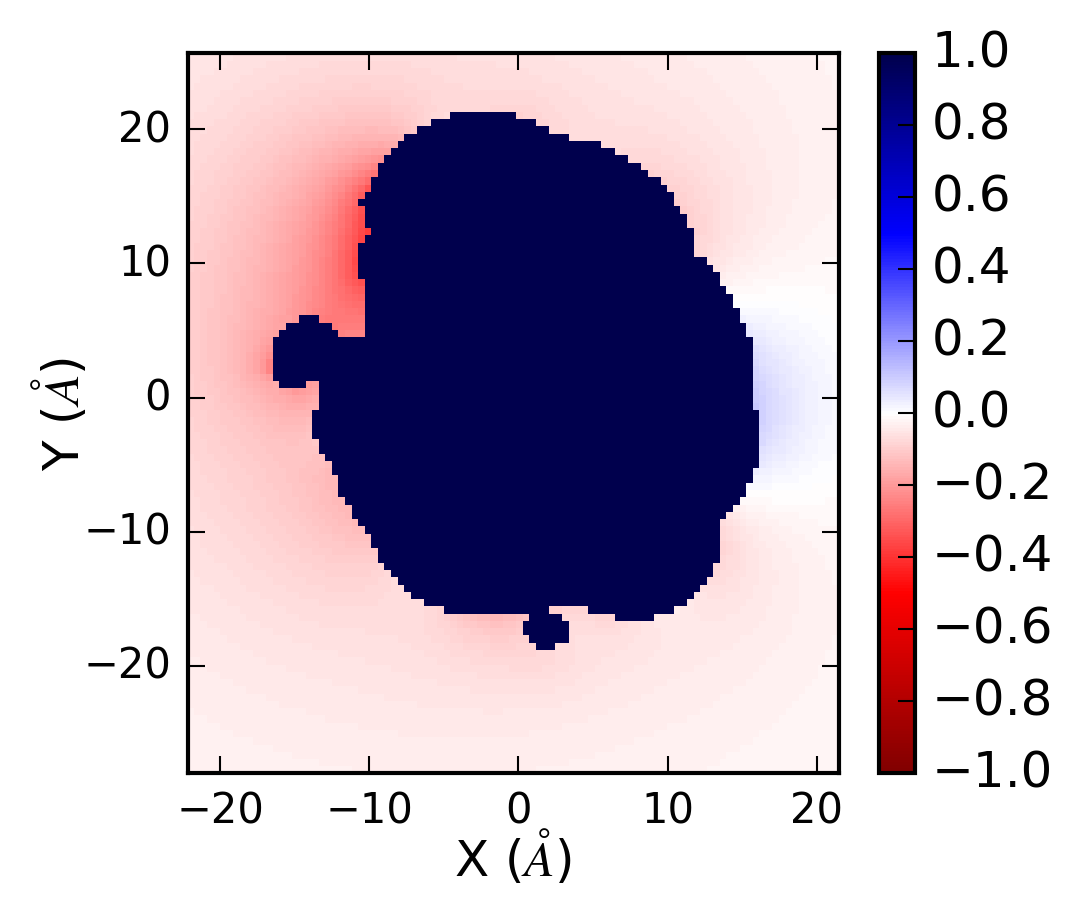
\includegraphics[width=0.32\linewidth]{pbsam_barstar} 
	(B)~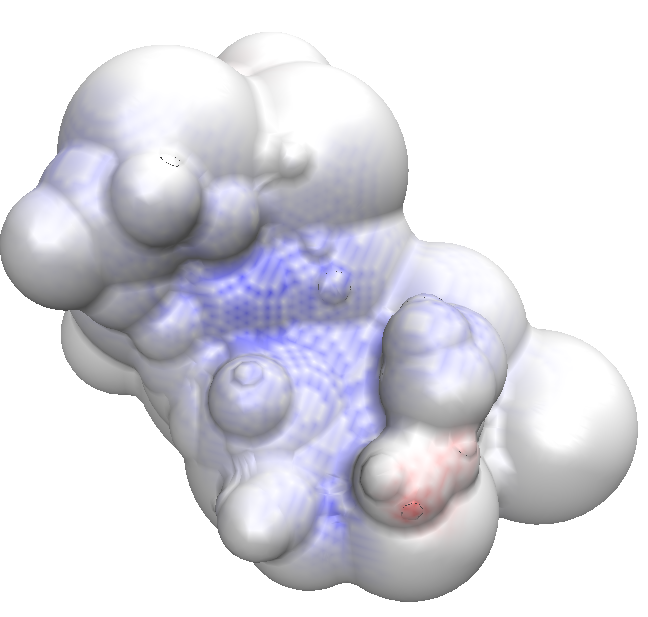
\includegraphics[width=0.30\linewidth]{pbsam_barnase} 
	(C)~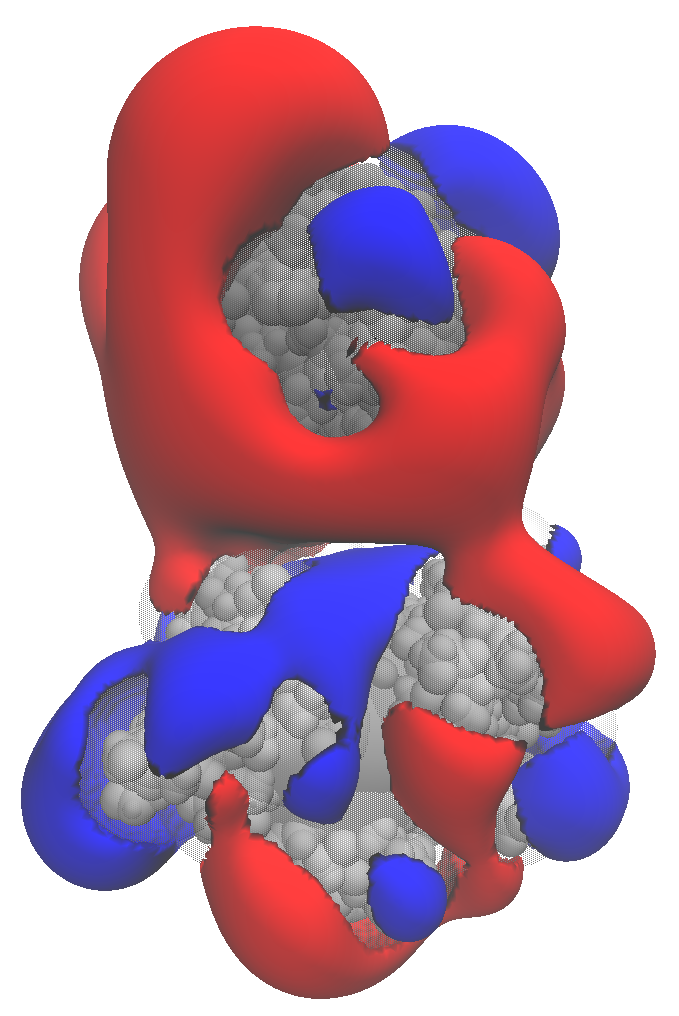
\includegraphics[width=0.20\linewidth]{pbsam_barnase_barstar}
	\vspace{-10pt}
	\caption{\small ESP results derived from APBS PB-SAM (0.0M salt, 7 pH, dielectric 2 (protein), and 78 (solution)): (A) potential in a 2D plane surrounding a barstar molecule (\(k_BT/e\)), 
		(B) potential on the coarse-grain surface of the barnase molecule (blue region
		is the location of barstar association, Max = 1.0 \(k_BT/e\), min = -1.0 \(k_BT/e\)), 
		(C) VMD visualization of the ESP around the association of barnase and barstar (molecules are given in grey and isosurfaces are drawn at 1.0 (blue) and -1.0 (red) \(k_BT/e\)).}
	\label{fig:pbsam-results}
	\vspace{-1em}
\end{figure}	

\paragraph{foo}


These methods use fast iterative techniques that solve a sparse linear system. However, issues have been identified which effect the results and performance of the models. The following issues were identified by Geng and Krasny \cite{geng2013} when solving the PB equation utilizing numerical methods:
%
\begin{itemize}
	\itemsep-0.25em
	\item the memory requirements for a three-dimensional grid can be prohibitively large,
	\item the geometric details of the molecular surface may be obscured on a regular grid,
	\item the singular atomic charges are smoothed by interpolation onto the grid,
	\item the interface conditions may not be rigorously enforced on the molecular surface., and
	\item the far-field boundary condition is often satisfied only approximately on a truncated domain.
\end{itemize}
%
To address these issues, new methods have been added to APBS to improve the flexibility for more diverse applications, address issues identified with grid-based methods, increase performance, and to expand the analysis capabilities of APBS. These methods are described in the following sections. For each method, we briefly discuss the algorithms that were implemented, how a user may use them, and show example results for several of the methods.





\subsubsection{Geometric Flow}
To increase the accuracy of our implicit solvent modeling, we have recently implemented a differential geometry based geometric flow solvation model. In this model, polar and nonpolar free energies are coupled through a characteristic function. This function describes a smooth dielectric interface profile across the solvent-solute boundary \cite{thomas2013}. 

For our modeling, a generalized form of the Poisson equation for computing the electrostatic is used as shown in Eq. \ref{eq:GFpoisson}, where $\epsilon_m$ and $\epsilon_s$ are the dielectric coefficients of the solute and solvent, respectively, and $\rho_m$ is the charge distribution of the fixed solute molecule. For this model, the solutions for the electrostatic potential ($\phi$) and the characteristic function ($S$) are obtained by minimizing the free energy functional. The dielectric function $\epsilon$($S$) takes on the value $\epsilon_m$ in the solute region ($S$=1) and the value $\epsilon_s$ in the solvent region ($S$=0).

\begin{equation}\label{eq:GFpoisson}
-\nabla \cdot\left(\epsilon\left(S\right)\nabla\phi\right)=S\rho_m
\end{equation}

For this model, we have utilized an Eulerian formulation of the geometric flow problem. This means that $S$ varies smoothly across the solute-solvent interfaces and leads to a non-linear partial differential equation for the characteristic function, $S$, as shown in Eq. \ref{eq:Spde}.

\begin{equation}\label{eq:Spde}
-\nabla\cdot\left(\gamma\frac{\nabla S}{\parallel\nabla S\parallel}\right)+p-\rho_0U^{att}+\rho_m\phi - \frac{1}{2}\epsilon_m\mid\nabla\phi\mid^2+\frac{1}{2}\epsilon_s\mid\nabla\phi\mid^2=0
\end{equation}
where $\gamma$ is the microscopic surface tension, $p$ is the hydrodynamic pressure, and $U^{att}$ is the attractive potential of the van der Waals dispersion interaction between the solute and the solvent.

The solution to this non-linear PDE can be solved by utilizing the parabolic PDE shown in Eq. \ref{eq:NLpde}. This equation is known as the generalized geometric flow equation and it is coupled with the Poisson equation through the characteristic function $S$ \cite{chen2010}.

\begin{equation}\label{eq:NLpde}
\frac{\partial S}{\partial t}=\gamma\parallel\nabla S\parallel\left[\nabla\cdot\left(\frac{\nabla S}{\parallel\nabla S\parallel}\right)+\frac{V}{\gamma}\right],
\end{equation}
where $V$ is known as the generalized flow potential as described in Eq. \ref{eq:flowpotential}. 

\begin{equation}\label{eq:flowpotential}
V=-p+\rho_0U^{att}-\rho_m\phi+\frac{\epsilon_m}{2}\mid\nabla\phi\mid^2-\frac{\epsilon_s}{2}\mid\nabla\phi\mid^2.
\end{equation}
%
These equations were solved using a second-order central finite difference scheme, which utilizes a bi-conjugate gradient stabilized solver.

The sensitivity and accuracy of an implicit solvent method typically depends on the values selected for the force-field parameters. However, the geometric flow method is only dependent on the parameters of the implicit solvent model (surface tension, dielectric coefficient, solvent pressure, etc.).

In a sensitivity analysis performed by Thomas et. al. \cite{thomas2013}, changing the distance between the axis boundary and the surface of each molecule and the grid spacing for the solver showed little effect on the results (3-5$\%$). However, changes in the internal dielectric ($\epsilon_m$) resulted in much larger sensitivity (i.e., changes in the results).

\subparagraph{Usage in APBS}
The differential geometry-based geometric flow solvation model is used to describe a smooth dielectric interface profile across the solvent-solute boundary in a thermodynamically self-consistent fashion. The main parameters of the model are the solute/solvent dielectric coefficients, solvent pressure on the solute, microscopic surface tension, solvent density, and molecular force-field parameters.

This model is accessed under the ELEC section of the input file. Results using the OPLS-AA force-field calculations, with and without van der Waals dispersion (vdW), are shown in Figure \ref{fig:geoflow} and were discussed by Thomas and friends \cite{thomas2013}. 
%
\begin{figure}
	\centering
	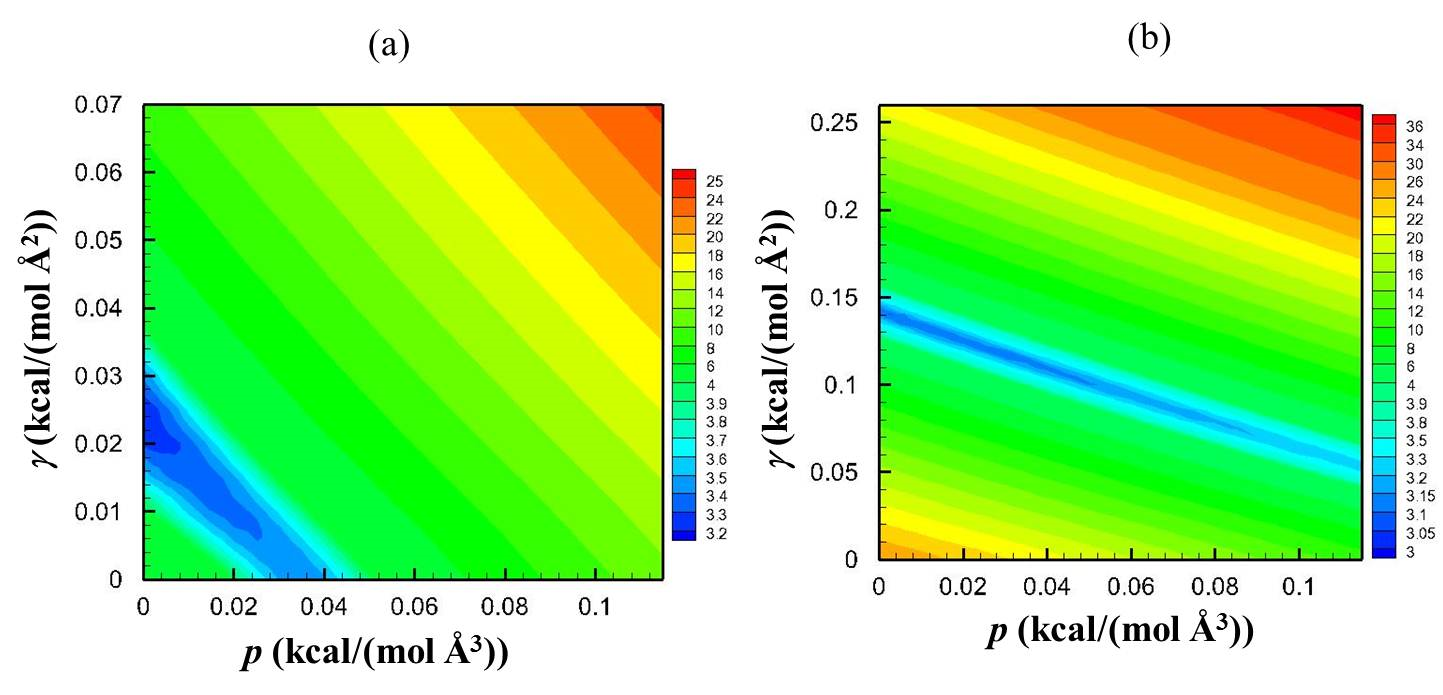
\includegraphics[width=0.80\linewidth]{geoflow.png} 
	\caption{Contour plot of the error between experimental and calculated solvation free energies based on OPLS-AA calculations:  (a) without vdW;  (b) with vdW.}
	\label{fig:geoflow}
\end{figure}

\subsection{Visualizing and using the results}
APBS was designed to facilitate use with other programs. This section outlines some of the programs with which APBS is known to work with. 

\subsubsection{Thick-client visualization}
%
\textbf{Graphical User Interfaces} 

PyMOL - molecular visualization and animation package which provides an interface to APBS. The APBS plugin to PyMOL permits isocontour and surface map visualization of APBS results.\footnote{www.pymol.org}

VMD - molecular visualization and animation package which provides an interface to APBS. It permits visualization of APBS results as isocontours, electric field lines, or on biomolecular surfaces. VMD also has graphical plugin to setup APBS calculations and execute them either locally or remotely via BioCoRE \cite{humphrey1996}. 

PMV - Python-based molecular visualization package which provides an interface to APBS. It not only permits visualization of APBS results but it also integrates setup and executation of APBS calculations.\footnote{www.mgltools.scripps.edu/packages/pmv}

Chimera - molecular visualization package which provides an interface to APBS.The APBS plugin integrated in Chimera allows the user to run a protein through both PDB2PQR and APBS to optimize the protein and view the electrostatic potential \cite{pettersen2004}. \\
%
\textbf{Visualization Software} \\
Electrostatic potentials are commonly visualized in the context of biomolecular structure to better understand functional aspects of biological systems. Note that the graphical user interfaces discussed above can also be used to visualize APBS output. The following molecular graphics software can display potentials and other data output from APBS:

Off-Target Pipeline - implements APBS to estimate ligand binding energies and compare electrostatic potential distributions within binding cavities \cite{evangelidis2012}.

Dino3D - molecular graphics program which can read UHBD-formatted electrostatic data. APBS can write multigrid results in UHBD format and therefore can be used with Dino3D.\footnote{www.dino3d.org}

OpenDX - general data visualization package which can read APBS output using the scripts provided in tools/visualization/opendx. However, as there is no straightforward way to visualize the potential in the context of the atomic structure, OpenDX should not be a first choice for APBS visualization.\footnote{www.opendx.org}

\subsubsection{Web-based visualization}
Computational chemists and biologists rely on molecular visualization tools to view model proteins and predict unobserved protein simulations~\cite{Jones2005}. These tools allow scientists to efficiently visualize and explore proteins. Thus allowing for a better understanding of relationships and functions of proteins.  

Visualization tools for evaluating simulation results are critical for the discovery of new insights.  Molecular viewers are available as stand-alone desktop programs or web-based applications. Desktop users are often burdened with obtaining software licenses or downloads when using desktop viewers such as VMD and web-based users are troubled with java security settings, permissions, or browser plug-ins when using web-based viewers such as Jmol~\cite{herraez2006}. While most viewers offer the same features such as rendering styles and coloring methods, lack of accessibility and poor performance can become a hindrance for scientists as they conduct research. 

To help with these issues, we have integrated 3Dmol~\cite{rego2015} into the PDB2PQR software and APBS pipeline. 3Dmol is a molecular viewer that offers the performance of a desktop application and convenience of a web-based viewer which broadens accessibility for all users. In order to integrate 3Dmol, enhancements were need for our tools, including extending our output file formats and creating a customized user interface. In the end, we have enabled a new light weight capability for visualization of complex electrostatic properties.

To allow users web-based access to PDB2PQR and APBS, we utilize  a web server interface hosted at the National Biomedical Computation Resource (NBCR)\footnote{www.nbrc.ucsd.edu} Center which uses the Opal2 toolkit to interface with the NBCR cluster. Opal2 handles the scheduling and execution of jobs and stores the results for later retrieval  \cite{krishnan2009}.  The NBCR server is designed to facilitate the setup and execution of continuum electrostatics calculation from PDB data, particularly by non-experts. The web service is driven by a modular Python-based collection of routines, which provides considerable flexibility to the software and permits non-interactive, high-throughput usage. 

We use the new capabilities in 3Dmol to render common molecular data representations for visualization and analysis.  Data from the APBS output file is used to generate surfaces, apply color schemes, and display different molecular styles such as cartoons and spheres. An example of the 3Dmol interface is shown in Figure \ref{fig:3dmol_interface}. The graphical user interface (GUI) has three surface options; solvent accessible, solvent excluded, and van der Waals. 

Using the GUI, the user can show or hide the surface or display it as translucent or opaque. The user can apply a minimum and maximum surface potential value. The default minimum and maximum isovalues are -5 kT/e and 5 kT/e, respectfully. The user can select a line, stick, cross, sphere, or cartoon model and apply a red-white-blue or red-green-blue color scheme to the surface. Additionally, 3Dmol renders proteins using different styles and color schemes, detailed in Table~\ref{tab:table1}.
Figure~\ref{fig:features} shows the visual representation of some selected features.

\begin{figure} 
	\begin{center}
		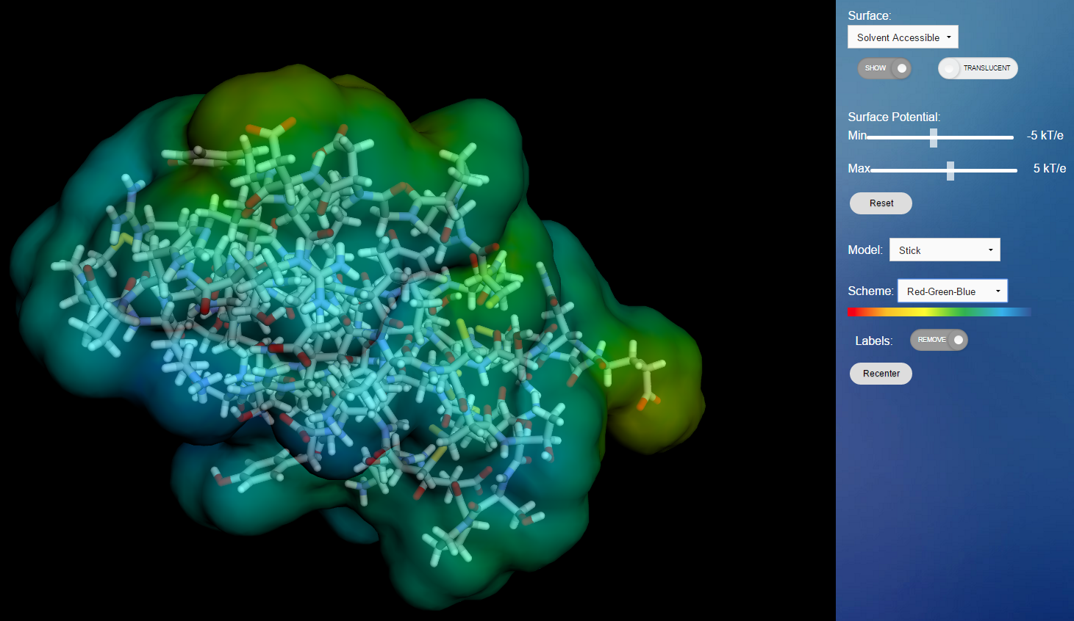
\includegraphics[width=.80\textwidth]{3dmol_interface.png}
		\caption{\small 3Dmol interface displaying a
			rendering of FASCICULIN (1FAS) protein with
			translucent, solvent accessible surface using a
			stick model and red-green-blue color scheme. 
			\color{black}  \label{fig:3dmol_interface}}  
	\end{center}  
\end{figure}

\begin{table}
	\small
	\begin{center}
		\caption{Selected 3Dmol features.}
		\label{tab:table1}
		\begin{tabular}{l l}
			Feature & Description\\
			Solvent accessible surface & describes the surface area of a biomolecule that is accessible to a solvent \\
			Red-White-Blue & describes the color scheme, red to white to blue, for charges \\
			Stick model & draws bonds as capped cylinders \\
			Cross model & draws atoms as crossed lines (i.e., stars) \\
			Sphere model & draws atoms as spheres \\
		\end{tabular}
	\end{center}
\end{table}

\begin{figure}
	\begin{center}
		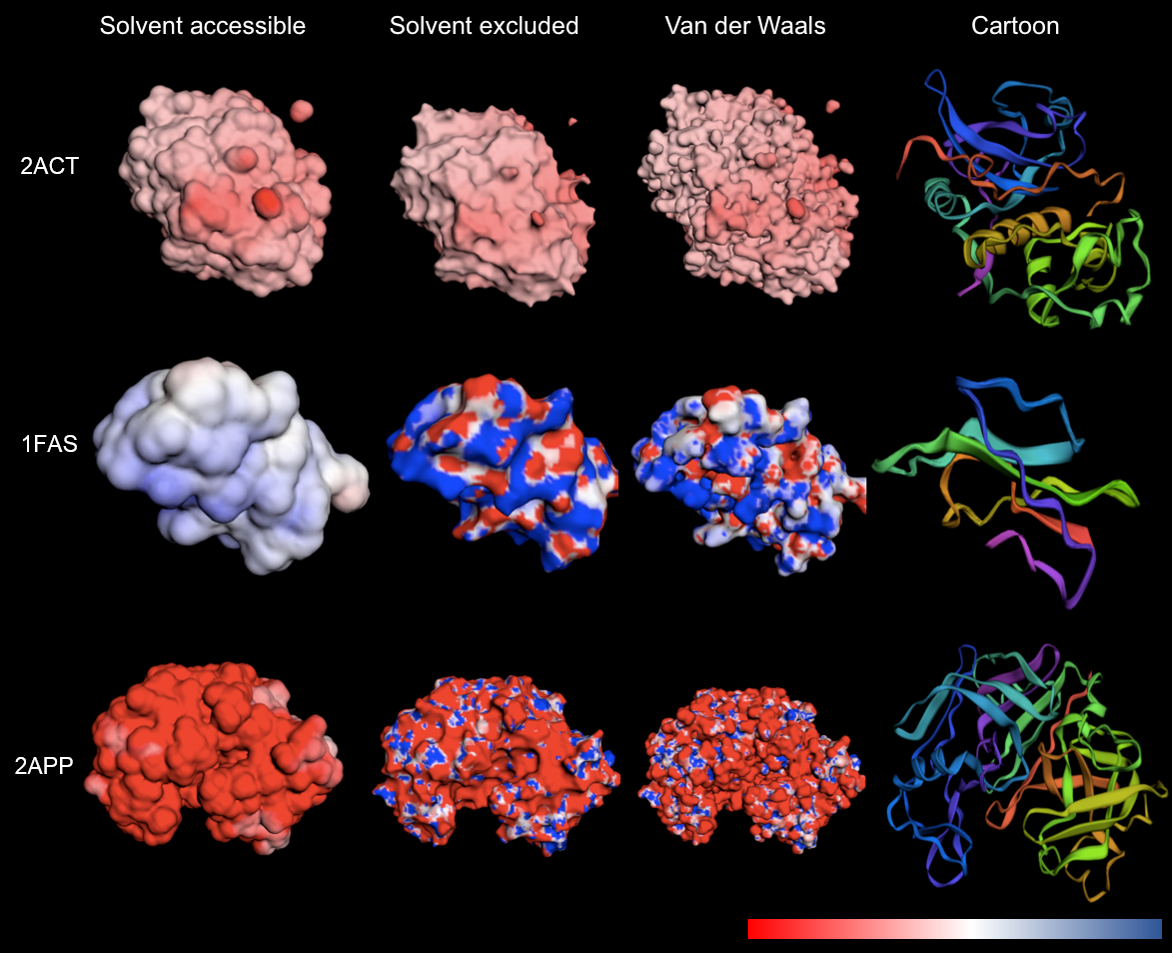
\includegraphics[width=.75\paperwidth]{features.png}
		\caption{\small Renderings of three different proteins using renderings of Actinidin (2ACT) (top), Fasciculin (1FAS) (center), and Pepsin, Penicillium (2APP) (bottom). To demonstrate the different  visualization options. From left to right, solvent accessible surface, solvent excluded surface, van der Waals  surface, and cartoon model are shown all using red-white-blue color scheme (excluding cartoon model). 
			\label{fig:features}}  
	\end{center}  
\end{figure}

3Dmol is an effective, interactive molecular viewer that is accessible across web browsers and operating systems. With 3Dmol, users can make selections using a simple GUI such as select different surfaces, apply various models, and choose from different color schemes.  The features available in 3Dmol are comparable to Jmol\footnote{www.jmol.sourceforge.net}, a molecular visualization tool written in Java; however, there are also differences between the two tools. While Jmol offers trace, backbone, cartoon, and ball and stick models, 3Dmol offers cartoon, cross, line, sphere, and stick models. Unlike Jmol, 3Dmol loads quickly and does not require any downloads or plug-ins for use. 

\subsubsection{Other data uses}
There are a number of other applications of implicit solvent models to biomedical problems. For example, during the past four years, our APBS software has been used in the post-simulation energetic analyses of molecular dynamics trajectories \cite{dror2013}, understanding protein-nanoparticle interactions \cite{treuel2013, nienhaus2013, depaoli2014}, understanding nucleic acid-ion interactions \cite{lipfert2014, giambasu2014}, biomolecular docking \cite{roberts2013}, developing new coarse-grained protein models \cite{spiga2013}, setting up membrane protein simulations \cite{stansfeld2015}, etc. APBS also plays a key role in software packages from the Wade group, including PIPSA for protein surface electrostatics analysis \cite{richter2008} and SDA for simulation of protein-protein interactions through Brownian dynamics \cite{martinez2015}. Another application area for implicit solvent methods is in the evaluation of biomolecular kinetics where implicit solvent models are generally used to provide solvation forces (or energies) for performing (or analyzing) discrete molecular or continuum diffusion simulations with APBS in both of these areas \cite{dror2013, martinez2015, chen2007, song2004a, song2004b, elcock2004, mereghetti2012}.

\section{Using the software}
APBS was designed as a standalone system and also to facilitate use with other programs. This section outlines execution methods and some of the programs with which APBS is known to work with. All of these methods are described in depth on the APBS-PDB2PQR website.\footnote{www.poissonboltzmann.org}

\subsection{Command-line execution}
Most users will likely interact with APBS and PDB2PQR through web servers. However, it is also possible to install local versions. These local installations give a command line version of the  software that can be customized through a variety of extensions. Compiled from source, a local version can also provide a web server.

\subsection{Execution through other programs}
APBS can also be execuated from other programs. As an example, the following programs have had capabilities to run APBS:
%%%
\begin{itemize}
	\itemsep-0.25em
	\item PDB2PQR
	\item iAPBS - Robert Konecny (McCammon Group) has developed iAPBS, an interface between APBS and the simulation packages AMBER, CHARMM, and NAMD. The iAPBS package provides a C/C++ and Fortran interface to APBS through a single function call. The interface code can be compiled as a library (libiapbs.a) which can be linked with a Fortran or C/C++ application thus making most of APBS functionality available from within any C/C++/Fortran code. \footnote{www.mccammon.ucsd.edu/iapbs} 
	\item TINKER - APBS 1.3 is available with TINKER; TINKER is a molecular modeling software package for molecular mechanics and dynamics, and includes some special features for bioploymers.\footnote{www.dasherwustl.edu/tinker}
\end{itemize}

\subsection{Web-based execution}

As discussed earlier, web-based executation of APBS is accomplished using the Opal Toolkit produced by the NBCR. This toolkit allows for the computing load for processor intensive scientific applications to be shifted to a 3rd party and/or generic computing grid. This can be tremendously advantageous in situations where a large amount of computing power is not locally available, but is required, for the task at hand. In particular, many users have discovered that their local computational resources are insufficient for certain types of APBS calculations on large systems or at extremely high accuracy. This client removes this resource limitation by allowing users to run on clusters at NBCR. Recent developmental versions of APBS add optional support for the off-loading of APBS calculations to an Opal service. 
The APBS Opal support is in the form of a Python script  \texttt{ApbsClient.py} and is installed by default when following the installation procedure outlined elsewhere. The script has been tested on Python 2.5; newer/older versions of Python may or may be functional. As mentioned above, the basic invocation is the same as the main binary. The only difference is the executable, which is called  \texttt{ApbsClient.py}, rather than  \texttt{apbs}. This client should be installed by default when APBS is installed. 

\subsection{Extending APBS capabilities}
There are several challenges when working with large code bases. Careful planning must go into the design, especially if the program is to be extended. Ideally, one would like the ability to link new code, which extends functionality, without having to change the existing base code. However, this is rarely the case. In the best scenario, a few line changes may be required. On the other hand, if proper care has not been taken, large modifications may be unavoidable.

To help with modularity, several programming paradigms have been introduced over the years. Object Oriented Programming (OOP), the paradigm used in the design of APBS, focuses on principal objects. Classes are used to define objects with given characteristics and functionality. This gives rise to a natural hierarchical structure where subclasses share any number of characteristics with the main class. APBS works with atoms, that form residues, that form molecules, etc, which naturally lends itself to the OOP paradigm. The C programming language is known for fast performance but does not natively supports OOP. To overcome this drawback, APBS was written using a subset of ANSI C called Clean OO C style by Mike Holst \cite{holst2001}. 

The main APBS file takes inputs from the command line and initializes some of the variables necessary for I/O and passing data to the Routines manager. The Routines manager, in turn, creates atom objects and invokes whichever solver is to be used. The advantages of using Clean OO C becomes clear when adding new solver methods to APBS. Because of APBS' OOP style, all one must do is make Routines aware of the new method. As long as the new methods adhere to Clean OO C calling conventions, the passing and return of data is seamless and most other methods (e.g. reading and writing to DX files) can be used. New methods which are external or do not adhere to Clean OO C standards can be managed by writing auxiliary methods for translating data from one to the other. These auxiliary methods are given in a header and source file. The external methods are linked at compilation time.

\section{Future directions}
The focus of APBS and its accompanying software is the modeling of solvation and electrostatic properties of macromolecules in biomedical research. As such, continued research and development of APBS is focused on modeling different possible application scenarios that may arise in the modeling of the solvation and electrostatic properties. 

APBS contains many different models and methods, which gives it a unique capability as a software package to be utilized in many different research applications. Methods that have been examined for future implementation into APBS and PDB2PQR include: advanced methods (gPC) for quantifying the influence of uncertainty on simple solvation-related properties (such as solvent-accessible surface area), ensemble averaging methods for titration state predictions, and virtual reality visualization of electrostatic potentials and related properties.

Our vision for APBS is to build the infrastructure that can enable our users to implement their own models and methods so that they can run on a common system. Imagine all the duplication of effort in building UIs, file loaders, parsers, output writers, etc. All that could be eliminated. 

Our goal is to have a well designed, well tested and well documented industry grade framework that will make it possible for all of these various bimolecular software packages to work together. To leverage each other's capabilities, to exceed the sum of the individual software package capabilities.

\section{Acknowledgments}
The authors gratefully acknowledge NIH grant GM069702 for support of this research. PNNL is operated by Battelle for the U.S. DOE under contract DE-AC05-76RL01830.  

\bibliography{apbs}

\end{document}
